\documentclass[mastinf,utf8,bibnum,hyperref,zihtitle,german, lof, lot]{zihpub}
\usepackage[ruled,vlined,german,algochapter]{algorithm2e}
\usepackage{float}
\usepackage[table,xcdraw]{xcolor}
\author{Jan Philipp Simon Langen}
\title{Anwendung neuronaler Netze zur inhaltsbasierten Bildsuche bei historischen Bilddarstellungen}
\birthday{26. Dezember 1994}
\placeofbirth{Münsterlingen, Schweiz}
\betreuer{Dr. Christoph Lehmann \& Dr. Taras Lazariv}
\bibfiles{literatur}
\newcommand{\comment}[1]{}
\setlength{\emergencystretch}{1pt}
\abstractde{
\onehalfspacing
Die inhaltsbasierte Bildersuche erlaubt es, eine Suchanfrage aus den Pixelinformationen eines Bildes zu formulieren, um einen Datensatz nach Aufnahmen zu durchsuchen, die ähnliche Inhalte darstellen. Eine Besonderheit hierbei ist, dass eine solche Suche nicht auf Metainformationen zu den zu durchsuchenden Bilder angewiesen ist. Dies macht inhaltsbasierte Suchsysteme attraktiv für Anwendungsfälle wie historische Aufnahmen, für welche solche Metadaten selten zur Verfügung stehen. In der vorliegenden Arbeit wird das auf einem neuronalen Netz aufbauende inhaltsbasierte Suchsystem DELF (DEep Local Features) analysiert. Dabei soll untersucht werden, ob sich das DELF-Verfahren für den Einsatz auf historischen Aufnahmen eignet. Außerdem sollen zentrale Parameter des DELF-Verfahrens analysiert und für den Anwendungsfall der historischen Bilder optimiert werden.\\
Hierfür wird zunächst eine breit angelegte Parameteranalyse durchgeführt, in der eine Vielzahl unterschiedlicher Parameterkonfigurationen miteinander verglichen wird. Dabei werden die unterschiedlichen Konfigurationen sowohl auf einem Datensatz von historischen Aufnahmen wie auch auf einem bekannten Benchmarkdatensatz getestet. Somit können Zusammenhänge zwischen den unterschiedlichen Parametern sowie Einflüsse der historischen Domäne aufgedeckt werden. Um die Ergebnisse des parameter-optimierten DELF-Verfahrens auf dem historischen Datensatz einzuordnen, werden diese mit den Ergebnissen eines weiteren inhaltsbasierten Suchsystems (ConvNet) verglichen.
\\
Im Zuge der vorliegenden Arbeit werden die Einflüsse auf die Suchergebnisse mehrerer DELF-Parameter aufgezeigt und erläutert. Im abschließenden Verfahrensvergleich erreicht das DELF-System signifikante Verbesserungen gegenüber dem ConvNet-Verfahren. Somit bestätigt sich, dass das DELF-Verfahren für einen Einsatz auf historischen Aufnahmen eignet ist.
}

\abstracten{In content-based image retrieval (CBIR) the pixel content of an image is used as a query to search a database for images displaying similar contents. Hereby the search system solely relies on the image content, therefore no additional metadata is needed to conduct a search. This makes CBIR especially useful in search domains like historical images, where metadata such as tags, titles or location information is not available. In the presented work the application of a deep learning CBIR-system called DELF (DEep Local Features) as an image search system used on a large historical image dataset is evaluated. The goal hereby is to determine whether the usage of DELF is generally suitable and how the parameters of the DELF system should be set to optimize performance in this specific setting.\\
In order to achieve this at first a large number of experiments using different parameter configurations is conducted on a historical dataset as well as on a benchmarking dataset for image retrieval systems to gather information about the influences on the retrieval performance of the individual analysed parameters and the specific kind of illustrations found in the historical domain. To answer the question of suitability the retrieval results of the DELF-system on the historical dataset are compared with the results of a different deep learning CBIR-System named ConvNet.\\
In the course of the presented work a number of dependencies between different parameters and their influences on performance are revealed and explained. The DELF-System shows distinct improvements compared with the ConvNet-approach. Therefore it can be concluded that DELF is a suitable image retrieval system for the application within the historical image domain.}
\begin{document}
\setlength{\emergencystretch}{1pt}
\section*{Motivation}
Präzise und effiziente Suchwerkzeuge sind essenziell um große Datenmengen für einen Nutzer sinnvoll verwertbar zu machen. Dies gilt insbesondere auch im Bereich der Bildersuche. Die klassische Bildersuche basiert auf vom Nutzer formulierten Anfragen, mit deren Hilfe das Suchsystem eine Liste an passenden Bildkandidaten zusammenstellt und zurückgibt. Hierbei nutzt das System eine Reihe von Zusatzinformationen, sogenannten Metadaten, wie Tags, Titel, Aufnahmeort oder Datum. Eine alternativer Ansatz der Suche, der in dieser Arbeit behandelt wird, ist die inhaltsbasierte Bildersuche (engl. Content-Based Image Retrieval, kurz CBIR). Hierbei werden vom Nutzer keine Anfragen formuliert. Stattdessen dient ein Bild als Suchanfrage. Ziel ist es, Bilder mit gleichem oder ähnlichem Bildinhalt als Ergebnis zurückzugeben. Ein Vorteil dieser Herangehensweise ist, dass der Nutzer keine Informationen über den Inhalt des Suchbildes benötigt. Das System arbeitet ausschließlich mit den Pixelinformationen der Bilder. Ein weiterer Vorteil ist daher, dass weder im Suchbild noch in der Suchdatenbank Metadaten zu den Bildern vorhanden sein müssen, was die Einsatzmöglichkeiten von inhaltsbasierter Suche sehr flexibel gestaltet. Im Folgenden wird die inhaltsbasierte Suche auch als Image Retrieval bezeichnet.
\\\\
Das Anwendungsgebiet dieser Arbeit ist die Suche auf historischen Bildern. Diese weit gefasste Domäne ist besonders herausfordernd, da sie sehr heterogene Daten enthält. Dabei gibt es nicht nur große Unterschiede in den abgebildeten Bildinhalten, wie Gebäude, Naturaufnahmen oder Portraits, sondern auch in den verwendeten Aufnahmeverfahren. Durch die Fortschritte der Aufnahmetechnik können historische Bilder sowohl in Form von Zeichnungen oder Malerei, aber auch als Druck oder in anfänglichen Formen der Photographie vorliegen. Da Metadaten zu historischen Bildern erst bei der Digitalisierung hinzugefügt werden können, sind diese oft gar nicht oder nur lückenhaft vorhanden. Dies macht die inhaltsbasierte Suche für diese Domäne im Vergleich zur klassischen Bildersuche zu einer besonders geeigneten Methode. Mit der Umsetzung einer unterstützenden Suche für das UrbanHistory4D Projekt \cite{urbanhistory4d} ergibt sich ein konkreter Anwendungsfall für diese Arbeit. Das UrbanHistory4D Projekt befasst sich mit der Erstellung interaktiver Stadtkarten. Wo vorhanden kann sich der Nutzer historische Aufnahmen anzeigen lassen, die den Ort zeigen, an dem er sich innerhalb der Karte befindet. Das Akkumulieren und Zuordnen von historischen Bildern zu diesen Plätzen ist ein wesentlicher Arbeitsanteil bei der Erstellung der Karten. Image Retrieval Systeme können helfen den Suchaufwand für die Ersteller der Karten signifikant zu reduzieren. Dabei handelt es sich um einen aktiven Forschungsbereich, in dem momentan unterschiedliche Suchsysteme analysiert werden. 
\\\\
Das Image Retrieval Verfahren DELF (attentive DEep Local Features) \cite{delf} entwickelt von Noh, \mbox{Araujo} et al., welches in dieser Arbeit untersucht wird ist ein Deep Learning Ansatz. Durch den raschen Fortschritt im Bereich tiefer neuronaler Netzwerkarchitekturen der letzten Jahre erfreuen sich gelernte Ansätze immer größerer Beliebtheit. DELF erzielt auf bekannten Benchmarkdatensätzen wie Oxford5k \cite{oxford5k} und Paris6k \cite{paris6k} sehr gute Ergebnisse. Besonders gut schneidet DELF im Vergleich auf dem eigens erstellten Google Landmarks Datensatz \cite{landmarks} ab. Dieser enthält mit über 1 Mio. Bilder und 13k unterschiedlichen Motiven eine deutlich heterogenere Mischung an Objekten als andere Benchmarks. Die gute Performanz auf diesem Datensatz lässt also hoffen, dass sich das DELF-Verfahren auch für die historische Domäne eignet.



\chapter{Verwandte Arbeiten}\label{related_work}
Bei Information Retrieval handelt es sich um ein Problem aus dem Bereich der Computer Vision, welches bereits seit langem intensiv erforscht wird. In frühen Ansätzen versuchte man vor allem globale Beschreibungen von Bildern zu erstellen, um diese untereinander vergleichen zu können. Diese basierten zum Beispiel auf Farbhistogrammen oder Texturbeschreibungen \cite{early_days}. Allerdings waren diese Ansätze oft sehr anfällig für Unterschiede in Beleuchtung, Skalierung und anderen Transformationen, wie sie bei unterschiedlichen Aufnahmen des selben Motivs auftreten können.
\\
Ein wesentlicher Durchbruch gelang David G. Lowe 2004 mit der Entwicklung des SIFT-Verfahrens (Scale Invariant Feature Transform) \cite{sift}. Hierbei werden mehrere Konzepte vereint um Bildbeschreibungen zu erzeugen, die robuster gegenüber unterschiedlichen Transformationen sind. So arbeitet der SIFT Algorithmus beispielsweise nicht direkt auf den Bildern, sondern im sogenannten Scale Space. Dieser besteht auf unterschiedlich skalierten Versionen des Ursprungsbildes, auf welche wiederum unterschiedlich starke Gauß-Filter angewendete werden. Betrachtet werden schließlich Differenzbilder zwischen benachbarten Stärken der Gauß-Fitler Ergebnisse. Die Verwendung von unterschiedlich skalierten Bildversionen macht die berechneten SIFT-Merkmale deutlich robuster gegen Skalierungsunterschiede. Das SIFT-Verfahren besteht aus zwei Phasen. In der ersten Phase werden über die Suche nach lokalen Extrema bedeutsame Bildpunkte ausgewählt. Für diese werden in der zweiten Phase einzelne Deskriptoren berechnet. Das Bild wird also nicht global beschrieben, sondern über viele lokale Deskriptoren dargestellt. Die lokalen Deskriptoren ergeben sich aus Histogrammen der Gradientrichtungen umliegender Bildpunkte. Diese werden relativ zu der dominanten Gradientrichtung in der Umgebung berechnet, was die Deskriptoren invariant gegenüber Rotationen macht. Lowes Entwicklung bildet den Ursprung für viele abgeleitete Verfahren wie SURF\cite{surf}, PCA-SIFT\cite{pca_sift} und RIFT\cite{rift}. Auch in aktueller Forschung werden Image Retrieval Verfahren untersucht, die mit SIFT-Merkmalen arbeiten \cite{modern_sift_useage}. \\
Der Trend bei der Entwicklung neuer Image Retrieval Systeme geht aktuell jedoch hauptsächlich in Richtung von gelernten Verfahren. Die Basis dieser Verfahren bilden tiefe CNN-Architekturen (Convolutional Neural Networks). Ein neuronales Netzwerk lässt sich als eine schichtweise Aneinanderreihung nicht-linearer Funktionen auffassen. Convolutional Neural Networks sind ein Sonderfall neuronaler Netze, welche sogenannte Convolutional Layer, zu deutsch faltende Schichten, enthalten. In diesen Schichten werden Faltungs/ bzw. Filteroperationen auf die Eingabedaten angewendet, um für das Netzwerk hilfreiche Merkmale in den Daten hervorzuheben. Dies ist durchaus vergleichbar mit den Filteroperationen, die im SIFT-Verfahren verwendet werden. Der Unterschied besteht jedoch darin, dass die Parameter der verwendeten Filtermasken sowie aller anderen Netzparameter nicht per Hand gewählt, sondern in einem Trainingsverfahren für den aktuellen Anwendungsfall optimiert werden. Der Entwickler bestimmt lediglich die grobe Architektur des Netzwerks, also die Anzahl, Größe und Reihenfolge der verwendeten Schichten sowie die Art der Operationen, die in ihnen durchgeführt werden. In Image Retrieval Systemen werden CNNs eingesetzt, um Bilddeskriptoren zu erstellen. Hierfür werden Zwischenergebnisse des Netzwerks, also die Ausgaben einer bestimmten Schicht genutzt. An welcher Stelle im Netzwerk die Deskriptoren entnommen werden ist dabei von entscheidender Bedeutung. Zeiler und Fergus haben in ihrer Studie zur Visualisierung von CNNs gezeigt \cite{extraction_point_meaning}, dass die früheren Schichten von CNNs typischerweise einfache Konzepte wie Kanten oder Ecken hervorheben. Mit wachsender Tiefe der betrachteten Netzwerkschicht steigt auch die Komplexität der Konzepte, die von den Ausgaben der Schicht beschrieben werden können.
\\\\
In dem in \cite{fc_extraction_neural_codes} beschriebenen Image Retrieval System von Babenko, Slesarev et al. wird als Modell ein CNN bestehend aus fünf faltenden gefolgt von drei vollvernetzten Schichten (im Englischen fully-connected layer) genutzt. Als Deskriptoren werden die Ausgaben der ersten bzw. zweiten vollvernetzten Schicht verwendet. In einer vollvernetzten Schicht hat jeder Wert der Eingabe Einfluss auf jeden Wert in der Ausgabe. Die Ausgaben solcher Schichten werden also von der gesamten Bildeingabe beeinflusst und können daher als globale Deskriptoren verstanden werden. Diese intuitive Herangehensweise erzielt leichte Verbesserung gegenüber den zur Zeit der Veröffentlichung gängigen algorithmischen Verfahren.
\\
Razavian, Sullivan et al. stellen in \cite{convnet} ein System auf Basis der in \cite{convnetarc} beschriebenen Netzwerkarchitektur vor. Das Modell besteht ebenfalls aus fünf faltenden und drei vollvernetzten Schichten. Die Deskriptoren stammen aus den Ausgaben der letzten faltenden Schicht.
%Die Dimensionalität der Deskriptoren wird durch Anwendung einer max-pooling Operation auf 2048 Dimensionen beschränkt.
Anders als bei Babenko, Slesarev et al. werden in diesem System mehrere Deskriptoren pro Bild erstellt. Hierfür werden systematisch Teilbilder aus Bildbereichen unterschiedlicher Größe generiert. Anschließend werden die Teilbilder auf eine feste Größe skaliert und als Eingabe in das Netzwerk gegeben. So wird für jeden betrachteten Bildbereich ein eigener lokaler Deskriptor erstellt. In ihren Experimenten stellen die Autoren fest, dass die Verwendung von lokalen Deskriptoren gegenüber einer globalen Betrachtung zu einer signifikanten Verbesserung der Retrievalperformanz führt. Der überwiegende Teil aktueller Retrieval Systeme setzt auf die Erstellung von lokalen Deskriptoren.
\\
Eine interessante Frage bei der Konzeption von Image Retrieval Systemen, die mit lokalen Deskriptoren arbeiten ist, wie man entscheidet, welche Bildregionen am sinnvollsten zu betrachten sind. Das ONE-Verfahren \cite{one} von Xie, Hong et al. nutzt ein VGG-19 \cite{vgg} Modell und extrahiert Deskriptoren aus der vorletzten vollvernetzten Schicht. Als Eingaben in das Netzwerk dienen sogenannte Object Proposals. Dabei handelt es sich um Bildausschnitte, welche Regionen umschließen, in denen Objekte vermutet werden. Die Autoren testen sowohl manuell annotierte sowie automatisch extrahierte Object Proposals und erzielen mit beiden Ansätzen ähnlich gute Ergebnisse. Für die automatische Bestimmung von Object Proposals nutzen sie das Selective Search Verfahren \cite{selective_search}.
\\
Das Delf-Verfahren \cite{delf}, welches in dieser Arbeit untersucht wird, basiert ebenfalls auf lokalen Deskriptoren. Die Deskriptoren werden aus einer faltenden Schicht aus dem hinteren Teil eines ResNet-50 \cite{resnet} Modells extrahiert. Als Eingabe in das Netzwerk werden Bilder in ihrer Gesamtheit betrachtet. Da bis zur Extraktionsschicht keine vollvernetzten Schichten genutzt werden, kann für jeden extrahierten Wert zurückgerechnet werden, von welchen Bereichen des Ursprungsbildes er beeinflusst wurde. Dies erlaubt es die Ausgaben der Extraktionsschicht in einzelne lokale Deskriptoren zu unterteilen. Um auszuwählen welche der lokalen Deskriptoren zur Darstellung eines Bildes genutzt werden sollen, werden die lokalen Deskriptoren in ein weiteres neuronales Netz gegeben. Dieses Netz hat die Aufgabe zu bewerten, wie geeignet die einzelnen Deskriptoren zur Beschreibung des Gesamtbildes sind. Auf Grund dieser Bewertung werden die wichtigsten Deskriptoren zu jedem Bild ausgewählt, wogegen schlecht bewertete Deskriptoren verworfen werden. Der konzeptionelle Unterschied bei der Auswahl der Deskriptoren im Vergleich zum ONE-Verfahren ist, dass die Auswahl auf Grund der bereits berechneten Deskriptoren geschieht anstatt auf Grund des Ursprungsbildes. Die Funktionsweise des Delf-Verfahrens wird in Kapitel \ref{delf_chapter} ab Seite \pageref{delf_chapter} im Detail erklärt.
\\  
Bevor Neuronale Netze für die Erstellung von Deskriptoren genutzt werden können, müssen ihre Parameter in einem Trainingsverfahren optimiert werden. Während dem Training muss das Netzwerk eine Aufgabe lösen. Wie erfolgreich das Netzwerk dabei ist, wird mit Hilfe einer Fehlerfunktion dargestellt. Das Netz versucht seine Parameter so anzupassen, dass die Fehlerfunktion minimiert wird. Im Fall der bereits vorgestellten Verfahren wird dabei eine Dummy-Aufgabe, typischerweise die Klassifikation von Bildern, gelöst. In der letzten Zeit wurden jedoch einige Ansätze veröffentlicht, die versuchen neuronale Netze direkt an Image Retrieval Aufgaben zu trainieren. Radenović, Tolias und Chum stellen in \cite{siamac_contrastive_loss} eine solchen Ansatz vor. Während dem Training arbeiten sie dabei mit Bildpaaren $(i,j)$. Diese Paare werden als korrektes Match bezeichnet, falls sich ihre Bildinhalte überschneiden. Andernfalls handelt es sich um ein inkorrektes Match. Beide Bilder durchlaufen ein identisches Netz und erzeugen dabei jeweils eine Ausgabe $(\mathbf{d}(i),\mathbf{d}(j))$. Für die Optimierung wird eine spezielle Fehlerfunktion $L$ definiert. Falls es sich bei den Bildern um ein korrektes Match handelt, sollten sich die Netzwerkausgaben der Bilder möglichst ähneln.
\begin{equation}
L_{korr}(i,j) = \dfrac{1}{2} \parallel \mathbf{d}(i) - \mathbf{d}(j)\parallel^{2} 
\end{equation}
Handelt es sich jedoch um ein inkorrektes Match, sollten die Ausgaben einen Mindestabstand $\tau$ zueinander einhalten.
\begin{equation}
L_{inkorr}(i,j) = \dfrac{1}{2} \max\left[0, \tau - \parallel \mathbf{d}(i) - \mathbf{d}(j)\parallel^{2}\right] 
\end{equation}
Die Autoren testen ihr Verfahren auf unterschiedlichen CNN Architekturen wie VGG \cite{vgg} und AlexNet \cite{alexnet} und erzielen damit sehr gute Ergebnisse auf gängigen Retrievalbenchmarks. Das direkte Training auf Retrievalaufgaben ist eine vielversprechende neue Forschungsrichtung im Retrievalbereich, an der momentan intensiv gearbeitet wird.
\\\\
% delf gesamtes bild als input durch conv layer wird auf lokale punkte zurückgerechnet. attention training auf den deskriptoren um gute auszuwählen. näheres  im konkreten kapitel
% diese system benötigen alle einen dummy task um die netzwerke zu trainieren oder benutzen vortrainierte netze alles mit klassifikation trainiert. es gibt aber ansätze die versuchen ein direkt für einen retrieval taks zu trainieren sia mac
Da Image Retrieval Systeme meist auf großen Bilddatenbanken eingesetzt werden und somit für eine Suchanfrage viele Bilder miteinander verglichen werden müssen, ist es sinnvoll Bildrepräsentationen so kompakt wie möglich zu gestalten, um die Laufzeit der Suche zu verbessern. Insbesondere bei Verfahren, die lokale Deskriptoren erstellen und häufig hunderte oder tausende Merkmale pro Bild extrahieren, kann mit einer guten Kodierung viel Rechenzeit gespart werden. Ein beliebter Ansatz zur Erstellung kompakter Darstellungen aus lokalen Deskriptoren ist das BOVW-Modell (Bag-of-Visual-Words) \cite{bow}, erstmals vorgestellt im Kontext von Textklassifikation von McCallum und Nigam. Hierbei werden zunächst alle aus einem Datensatz extrahierte Deskriptoren mittels Clusteranalyse (bspw. K-Means-Clustering \cite{k_means}) in Gruppen eingeteilt. Deskriptoren, die dem gleichen Cluster zugeordnet werden, werden dabei auf das selbe "visuelle Wort"\ abgebildet. Als Beschreibung des Gesamtbilds dient ein Histogramm über die im Bild enthaltenen visuellen Wörter. Bei diesem Verfahren geht durch Quantisierung ein Teil der Information verloren. Das ebenfalls auf Clustering basierte VLAD-Verfahren \cite{vlad} von Jégou, Douze et al. versucht diese Information nutzbar zu machen, indem es statt der Vorkommen die Quantisierungsfehler akkumuliert, die beim abbilden auf die nächsten visuellen Worte entstehen. \\
Um eine Suchanfrage mit einer Rangliste der ähnlichsten Bilder zum Suchbild beantworten zu können, werden die Deskriptoren der Bilder in der Datenbank mit denen des Suchbildes verglichen. Als Metrik dient hierbei meist die euklidische Distanz. Auf kleinen Datensätzen ist es laufzeittechnisch sinnvoll alle Kombinationen von Such- und Datenbankbildern zu vergleichen. Häufig werden bei größeren Datensätzen jedoch Methoden der approximierten nächsten Nachbarsuche (ANN) verwendet. Diese garantieren zwar kein optimales Ergebnis, erlauben jedoch deutlich schnellere Verarbeitung von Suchanfragen. So gibt es zum Beispiel Ansätze Deskriptoren mit Hilfe spezieller Hashfunktionen zu vergleichen. Diese werden so konstruiert, dass ähnliche Deskriptoren auf die gleichen bzw. möglichst ähnliche Hashcodes abgebildet werden, während gleichzeitig die Kollisionswahrscheinlichkeit für sehr unterschiedliche Deskriptoren minimal gehalten wird. Wang et al. beschreiben in ihrer Studie \cite{simsearch} unterschiedliche Konzepte für die Erstellung solcher Hashfunktionen.



%Den finale Teil einer Image Retrieval Pipeline bildet das Vergleichen der Anfragebilder mit den Bildern in der Suchdatenbank auf Basis der erzeugten Deskriptoren, mittels einer geeigneten Distanzmetrik (z.B. euklidische Distanz). Dabei ist ein erschöpfender Suchansatz auf Grund der Menge an Daten oft nicht sinnvoll. 




%Es gibt unterschiedliche Ansätze um das Problem der Suche nach den nächsten Nachbarn effizienter zu lösen. Ein Ansatz ist die Verwendung von räumlich partitionierenden Datenstrukturen, wie den von Friedman, Bentley und Finkel entwickelten K-D-Bäumen \cite{kd_tree}. Hierbei wird der Datenraum iterative entlang der unterschiedlichen Dimensionen der Elemente geteilt, wobei darauf geachtet wird, dass in den entstehenden Partitionen möglichst gleich viele Elemente enthalten sind. Dies wird solang wiederholt, bis in den einzelnen Partitionen nur noch eine geringe Anzahl an Elementen enthalten sind. Bei einer Suchanfrage 


\chapter{DELF}\label{delf_chapter}
Das Delf-Verfahren \cite{delf} von Noh, \mbox{Araujo} et al. bildet die Basis für die Experimente, die in dieser Arbeit durchgeführt werden. Im folgenden Abschnitt wird das Verfahren schrittweise im Detail erklärt. Beschrieben wird hierbei die Neuimplementierung in ihrer Basiskonfiguration, wie sie für den Experimentalteil dieser Arbeit verwendet wird. Unterschiede zu der von den Autoren zu Verfügung gestellten Implementierung\footnote[1]{\url{https://github.com/tensorflow/models/tree/master/research/delf}, zuletzt besucht 16.06.20}, sowie zu der Beschreibung des Verfahrens im Originalpapier \cite{delf} werden im hinteren Teil des Abschnitts erläutert. 
\\\\
Das Delf-Verfahren lässt sich in vier Phasen einteilen. Zu Beginn steht das sogenannte Finetuning. Hierbei wird ein vortrainiertes Modell, in unserem Fall ein ResNet-50 Netzwerk, auf einem neuen Datensatz weiter trainiert. Die Domäne der Bilder dieses Datensatzes sollte dabei möglichst nahe der späteren Retrievalaufgabe sein, damit das Modell lernen kann aussagekräftige Deskriptoren für diese Art von Bilden zu berechnen. In der nächsten Phase wird auf dem Modell aufbauend ein Attention-Netzwerk trainiert welches die Güte berechneter Deskriptoren bewertet. In der dritten Phase werden für die Bilder der Datenbank, in der gesucht werden soll Deskriptoren extrahiert. Mit Hilfe des Attention-Netzwerks wird eine Vorauswahl besonders geeigneter Deskriptoren getroffen. Anschließend durchlaufen die Deskriptoren weitere Vorverarbeitungsschritte, mit denen sie in eine kompaktere Form überführt werden. In der finalen Phase kann Delf aktiv genutzt werden. Es können nun Bilder als Suchanfragen gestellt werden. Delf vergleicht eine Anfrage mit allen Bildern des Datensatzes anhand der vorverarbeiteten Deskriptoren. Potentielle Matches zwischen Deskriptoren werden in einem letzten Schritt geometrisch verifiziert. Das Ergebnis einer Anfrage ist eine Rangliste der ähnlichsten Bilder, sortierte nach der Anzahl verifizierte Deskriptoren-Matches mit dem Anfragebild.

\section{ResNet}

Das Delf-Verfahren nutzt zur Erstellung von Deskriptoren ein Residuales Netzwerk (kurz ResNet). Bei der im Jahre 2015 vorgestellten ResNet Architektur \cite{resnet} von He, Zhang et al. handelt es sich um eine der meist genutzten tiefen CNN-Architekturen der aktuellen Forschung. ResNets finden Anwendung in unterschiedlichen Machine Learning Aufgaben, wie Klassifikation, Objektdetektion oder Image Retrieval. \\

Zeiler und Fergus haben gezeigt \cite{extraction_point_meaning}, dass CNNs mit wachsender Netzwerktiefe in der Lage sind komplexere Merkmale zu detektieren. Es scheint daher intuitiv zur Lösung immer komplexerer Aufgaben zunehmend tiefere Netzwerke zu konstruieren. Allerdings stellt sich heraus, dass ab einem gewissen Punkt keine Verbesserungen mehr mit dem bloßen aneinanderreihen von immer mehr Schichten erzielt werden können. Werden zu viele Schichten hinzugefügt kann die Trainingsperformanz sogar abnehmen. Mit dem rasanten Anstieg der Anzahl an Netzwerkparameter wird es immer schwieriger das Netzwerk zu optimieren. Parameter konvergieren deutlich langsamer zu einem Optimum und es gibt mehr lokale Minima in denen ein Netzwerk im Optimierungsprozess stecken bleiben kann. ResNets wirken diesem Problem mit der Einführung sogenannter Skip-Verbindungen entgegen. Hierbei werden zusätzliche Direktverbindungen im Netzwerk geschaffen, bei denen einige Schichten übersprungen werden. Fließt eine Eingabe an den Beginn einer Skip-Verbindung, so wird auf dieser die Identität der Eingabe mitgeführt. Parallel durchläuft die Eingabe die übersprungenen Schichten. Am Ausgangspunkt der Verbindung wird schließlich die Ausgabe der übersprungenen Schichten mit der Identität aufsummiert (siehe Abb. \ref{resnet}a). Durch die Bereitstellung der Identität hat das Netzwerk eine bessere Grundlage zur Optimierung und einzelne schlecht optimierte Schichten weniger negative Auswirkung auf die Netzwerkausgabe. Die Autoren stellen fest, dass CNNs bei Verwendung von Skip-Verbindung schneller zu einem Optimum konvergieren und dabei bessere Minima gefunden werden. 
\\
ResNets können in unterschiedlichen Konfigurationen erstellt werden. Das für Delf verwendete \mbox{ResNet-50} besteht aus 49 faltenden gefolgt von einer vollvernetzen Schicht. Skip-Verbindungen überspringen jeweils drei Schichten. Das Netzwerk kann in vier Blöcke unterteilt werden. Die Größe der einzelnen Featuremaps, der Ausgabe verringert sich nach jedem Block um den Faktor vier, wohingegen die Merkmalstiefe bzw. Anzahl der Featuremaps in der Ausgabe steigt (Siehe Abb.\ref{resnet}b). In der Implementierung dieser Arbeit wird die von Torchvision zur Verfügung gestellte ResNet-50 Architektur genutzt\footnote[2]{\url{https://github.com/pytorch/vision/blob/c2e8a00885e68ae1200eb6440f540e181d9125de/torchvision/models/resnet.py}, zuletzt besucht 16.06.20}. 
\begin{figure}
\label{resnet}
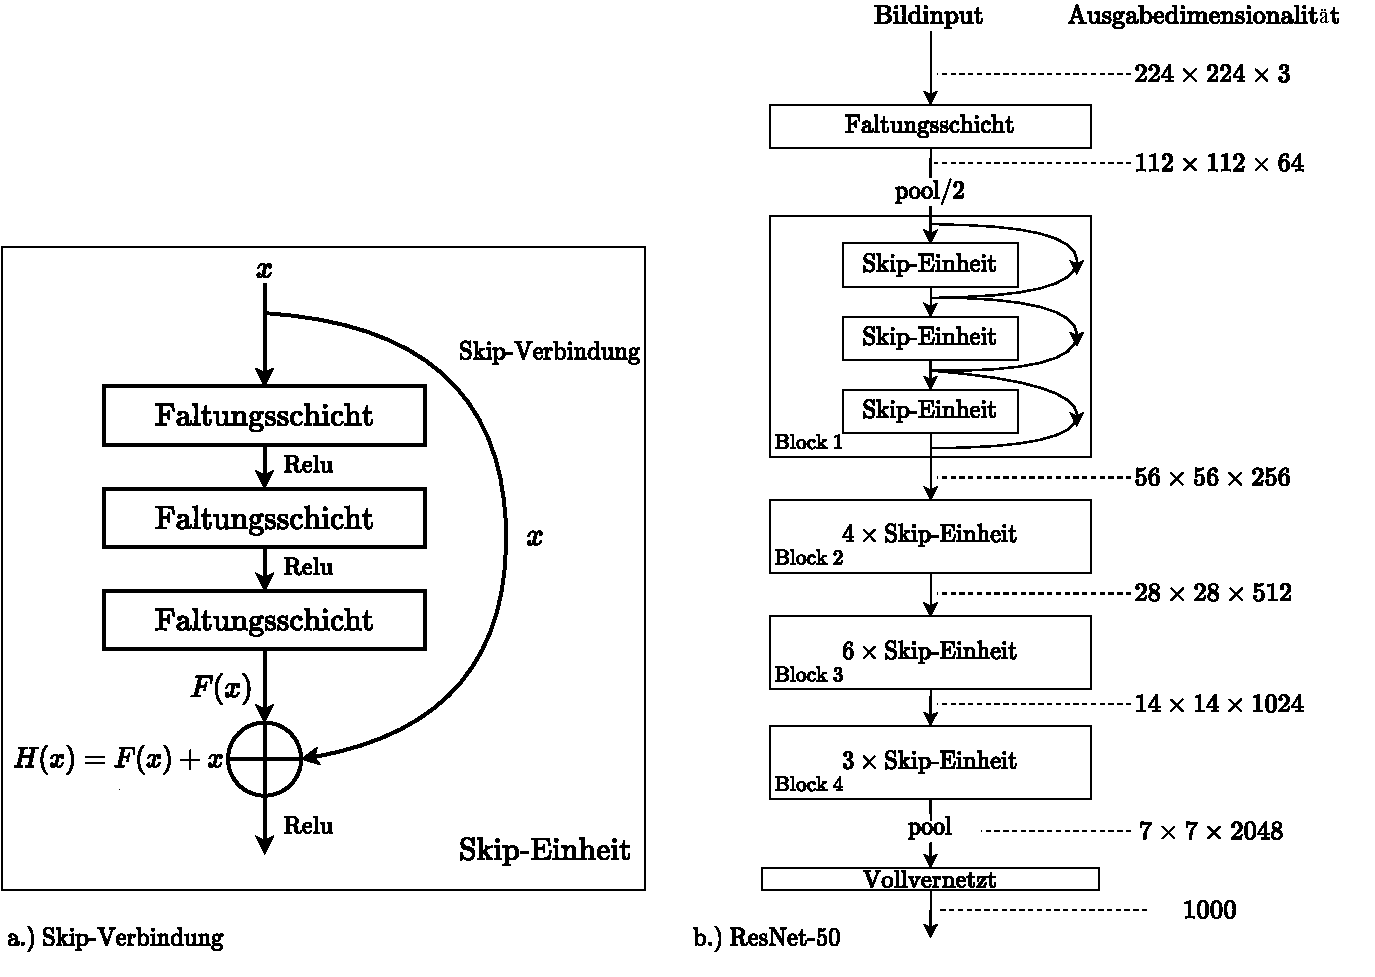
\includegraphics[scale=0.70]{resnet-50.pdf}
\caption{Aufbau der ResNet-Architektur (vgl. Fig.2, Fig.3 aus \cite{resnet})}
\end{figure}

\chapter{Evaluation}

Die Untersuchung des DELF-Verfahrens lässt sich in zwei wesentliche Abschnitte unterteilen. Zunächst werden in breit angelegten Experimentalreihen unterschiedliche Parameter innerhalb der DELF-Pipeline variiert, um ihren Einfluss auf die Ergebnisse der gelösten Retrievalaufgaben zu quantifizieren. Ziel ist dabei, sowohl ein besseres Verständnis für die Einflüsse einzelner Parameter zu schaffen, wie auch eine optimale Konfiguration für die Lösung von Retrievalaufgaben speziell für historische Bilder zu finden. \\
Im zweiten Abschnitt der Evaluation werden die Entscheidungen des optimierten DELF-Modells qualitativ untersucht, um ein besseres Verständnis für die Entscheidungsfindung des DELF-Prozesses zu erlangen. Insbesondere wird hier DELF mit anderen Retrievalverfahren verglichen, um Schwächen und Stärken des Verfahrens aufzudecken.

\section{Evaluationsdaten}

Zur Bewertung von Retrievalsystemen auf historischen Bildern steht ein eigens erstellter Datensatz zur Verfügung (vgl. Tab. \ref{hist4d_data}). Die 848 zusammengestellten Bilder umfassen historische Abbildungen von sieben Dresdner Sehenswürdigkeiten und entstammen vorwiegend den Archiven der deutschen Fotothek\footnote{\url{https://www.slub-dresden.de/sammlungen/deutsche-fotothek/}, zuletzt besucht am 02.09.20}. Auf Grund der geographischen Nähe einiger Sehenswürdigkeiten sind auf einigen Bildern des Datensatzes mehrere Objekte abgebildet. Bei der Auswertung gelten Bilder für alle Anfragen als korrekte Rückgabe, die mindestens ein Objekt zeigen, welches im betrachteten Bild zu erkennen ist. Bilder die auch als Suchanfrage verwendet werden sind immer genau einer Sehenswürdigkeit zuzuordnen.\\
\begin{table}[h]
\centering

\begin{tabular}{l|c|c|c|c|c|c|c}
\rowcolor[HTML]{C0C0C0} 
Objekt &
  \multicolumn{2}{c|}{\cellcolor[HTML]{C0C0C0}Zwinger} &
  \multicolumn{2}{c|}{\cellcolor[HTML]{C0C0C0}Hofkirche} &
  \multicolumn{2}{c|}{\cellcolor[HTML]{C0C0C0}Frauenkirche} &
  Semperoper \\
Anzahl Objektimpressionen & \multicolumn{2}{c|}{374} & \multicolumn{2}{c|}{216} & \multicolumn{2}{c|}{206} & 89    \\
Anzahl Anfragen           & \multicolumn{2}{c|}{6}   & \multicolumn{2}{c|}{8}   & \multicolumn{2}{c|}{7}   & 7     \\ \hline
\rowcolor[HTML]{C0C0C0} 
Objekt &
  \multicolumn{2}{c|}{\cellcolor[HTML]{C0C0C0}Sophienkirche} &
  \multicolumn{2}{c|}{\cellcolor[HTML]{C0C0C0}Stallhof} &
  \multicolumn{2}{c|}{\cellcolor[HTML]{C0C0C0}Moritzburg} &
  Total \\
Anzahl Objektimpressionen & \multicolumn{2}{c|}{66}  & \multicolumn{2}{c|}{38}  & \multicolumn{2}{c|}{23}  & 1012  \\
Anzahl Anfragen           & \multicolumn{2}{c|}{6}   & \multicolumn{2}{c|}{4}   & \multicolumn{2}{c|}{4}   & 42    \\ \hline
\rowcolor[HTML]{C0C0C0} 
Impressionen pro Bild     & \hspace{2.5mm} 0 \hspace{2.5mm}         & 1           & \hspace{1.1mm} 2 \hspace{1.1mm}           & 3          & \hspace{2mm} 4 \hspace{2mm}           & 5          & Total \\
Anzahl Bilder             & 0          & 730         & 81          & 29         & 7           & 1          & 848  
\end{tabular}%

\caption{Aufbau des historischen Datensatzes}
\label{hist4d_data}
\end{table}
Vorabexperimente haben gezeigt, dass die von DELF durchgeführte Deskriptorselektion nur befriedigende Ergebnisse liefert, wenn die verwendeten Bilder eine Mindestgröße einhalten. Im Selektionsschritt wählt das Attention-Netzwerk eine feste Anzahl an Deskriptoren. Da die Anzahl an extrahierten Deskriptoren je Bild mit der Bildgröße skaliert kann es bei sehr kleinen Bildern passieren, dass das Attention-Netzwerk alle, oder ein Großteil der extrahierten Deskriptoren auswählt. In diesem Fall findet keine bedeutsame Auswahl an Deskriptoren statt und der positive Effekt des Selektionsprozesses geht verloren (siehe Abb. \ref{small_img}).
\begin{figure}[h]
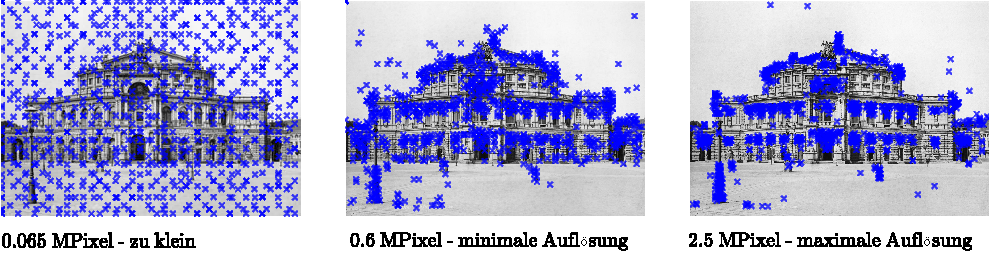
\includegraphics[scale=0.955]{scale_descriptor_selection.pdf}
\caption{Referenzpunkte der ausgewählten Deskriptoren bei unterschiedlicher Eingangsauflösung.}
\label{small_img}
\end{figure}
Auch sehr große Bilder können zu Problemen führen. Da die Bilder während dem Extraktionsprozess in mehreren Skalen betrachtet werden, können bei sehr großen Bildern Speicherproblem auftreten. Aus diesem Grund wird für die Bilder des Datensatzes eine minimale Auflösung von $0.6$MPixel und eine maximale Auflösung von $2.5$MPixel gefordert. Bilder die diese Restriktionen über- bzw. unterschreiten, werden auf die Maximal- bzw. Mindestgröße skaliert.\\
Neben historischen Daten wird das DELF-Verfahren zusätzlich auf dem Oxford5k-Datensatz \cite{oxford5k} getestet (vgl. Tab. \ref{oxford5k_data}). Hierbei handelt es sich um einen häufig verwendeten Benchmarkdatensatz, bestehend aus $5063$ Bildern. Das Bildmaterial entstammt Suchanfragen zu $11$ unterschiedlichen Sehenswürdigkeiten in und um Oxford, an die Fotocommunity Flickr\footnote{\url{https://www.flickr.com/}, zuletzt besucht am 03.09.20}. Häufig finden sich dabei Bilder von Personen oder Aufnahmen von Innenräumen, die keine der gesuchten Sehenswürdigkeiten abbilden. Diese Störbilder können entweder als zusätzliche Herausforderung angesehen oder aber vorab aussortiert werden. In den in dieser Arbeit durchgeführten Experimenten sind diese Störbilder im Datensatz enthalten. 
\begin{table}[h]
\centering
\begin{tabular}{l|c|c|c|c}
\rowcolor[HTML]{C0C0C0} 
Objekt                 & Radcliffe Camera & Christ Church & All Souls   & Magdalen \\
Anzahl Objektimpressionen & 348              & 133           & 111         & 103      \\
Anzahl Anfragen           & 5                & 5             & 5           & 5        \\ \hline
\rowcolor[HTML]{C0C0C0} 
Objekt                & Hertford         & Ashmolean     & Bodleian    & Balliol  \\
Anzahl Objektimpressionen & 61               & 31            & 30          & 18       \\
Anzahl Anfragen           & 5                & 5             & 5           & 5        \\ \hline
\rowcolor[HTML]{C0C0C0} 
Objekt                 & Cornmarket       & Keble         & Pitt Rivers & Total    \\
Anzahl Objektimpressionen & 13               & 11            & 8           & 867      \\
Anzahl Anfragen           & 5                & 5             & 5           & 55       \\ \hline
\rowcolor[HTML]{C0C0C0} 
Impressionen pro Bild     & 0                & 1             & 2           & Total    \\
Anzahl Bilder             & 4218             & 823           & 22          & 5063    
\end{tabular}%
\caption{Aufbau des Oxford5k Datensatzes}
\label{oxford5k_data}
\end{table}

\section{Retrievalmetriken}

Obwohl sich Klassifikations- und Retrievalaufgaben im Kern ähneln, können viele Metriken mit denen Klassifikationssysteme üblicherweise bewertet werden, wie beispielsweise Genauigkeit, nicht verwendet werden, um die Performanz von Retrievalsystemen zu evaluieren. Generell lassen sich aus der Betrachtung einzelner Bildpaare bestehend aus Anfragebild und Bildern des Suchindexes keine Rückschlüsse über die Performanz von Retrievalsystems ziehen.  Grundlage der Bewertung sind stets die gesamten Antworten des Retrievalsystems auf eingehende Suchanfragen. Entscheidend sind hierbei die Rankings, bzw. die Reihenfolgen in der die Bilder des Suchindexes auf die Anfragen zurückgegeben werden. Eine Möglichkeit diese Reihenfolgen zu bewerten ist die Erstellung sogenannter ROC-Kurve (Reciever-Operating-Characteristic)(vgl. Abb. \ref{metric_curve}a). Hierfür wird jeweils eine wachsender Anteil der zurückgegeben Bilder betrachtet und das Verhältnis zwischen Richtig-Positiv-Rate bzw. Recall und Falsch-Positiv-Rate dargestellt. Der Recall gibt an, welcher Anteil an Bildern mit gewünschten Bildinhalt bereits im betrachteten Abschnitt der Rückgabe enthalten war.
\begin{equation}
\text{Recall} = \frac{|\text{Bereits züruckgebene Bilder mit gewünschtem Inhalt}|}{|\text{Im Datensatz enthaltene Bilder mit gewünschtem Inhalt}|}
\end{equation}
Analog beschreibt die Falsch-Positiv-Rate den Anteil der Bilder ohne gewünschten Bildinhalt, der bereits zurückgegeben wurde.
\begin{equation}
\text{Falsch-Positiv-Rate} = \frac{|\text{Bereits züruckgebene Bilder ohne gewünschtem Inhalt}|}{|\text{Im Datensatz enthaltene Bilder ohne gewünschtem Inhalt}|}
\end{equation}
\begin{figure}[h]
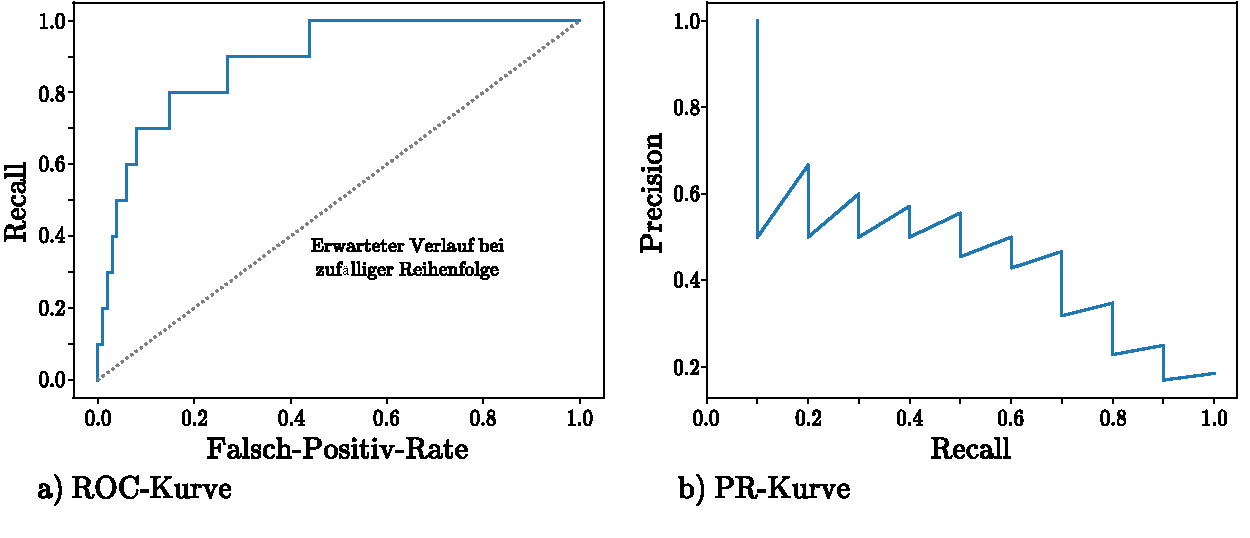
\includegraphics[scale=0.76]{metric_curves.pdf}
\caption{Vergleich von Kurvenmetriken einem Beispielsranking}
\label{metric_curve}
\end{figure}
\\
ROC-Kurven beginnen stets im Ursprung, wo noch keine Bilder zurückgegeben wurden und enden im Punkt $(1,1)$ wo der gesamte Datensatz zurückgegeben wurde. Die Gerade zwischen diesen Punkten bildet den erwarteten Verlauf, wenn das System Bilder in einer zufälligen Reihenfolge zurückgibt. Ein Retrievalsystem hat nur dann einen positiven Effekt für den Nutzer, wenn die ROC-Kurven ihrer Anfrageantworten oberhalb dieser Linie verlaufen. Obwohl ROC-Kurven gut in der Lage sind den Unterschied eines Suchsystems gegenüber einer zufälligen Suche aufzuzeigen, vermitteln sie aus der Perspektive eines tatsächlichen Anwenders oft ein zu positives Bild der Ergebnisse. Das liegt daran, dass der Anteil der Bilder, die für eine Anfrage relevant sind meist um ein vielfaches kleiner ist als der Anteil der irrelevanten Bilder, was an einer ROC-Kurve jedoch nicht ablesbar ist. Angenommen für eine Suchanfrage sind $10\%$ eines durchsuchten Datensatzes tatsächlich relevant und die zur Anfrageantwort erstellte ROC-Kurve zeigt bei einem Recall von $90\%$ eine Falsch-Positiv-Rate von $30\%$. Obwohl der Verlauf der Kurve ein sehr gutes Ergebnis suggeriert, sind für den Nutzer $75\%$ der zurückgegebenen Bilder irrelevant, die er gesehen hat, bevor ein Recall von $90\%$ erreicht wurde. Eine Möglichkeit, die tatsächliche Nutzererfahrung besser abzubilden ist die Erstellung von sogenannten PR-Kurven (Precision-Recall) (vgl. Abb. \ref{metric_curve}b). Hierbei wird die Präzision, also der Anteil der relevanten Bildern in der bisherigen Rückgabe gegen den Recall abgebildet.
\begin{equation}
\text{Precision} = \frac{|\text{Bereits züruckgebene Bilder mit gewünschtem Inhalt}|}{|\text{Bereits züruckgebene Bilder}|}
\end{equation}
So kann direkt abgelesen werden, welchen Anteil an irrelevanten Bildern innerhalb der Rückgabe toleriert werden müssen, um einen bestimmten Anteil der gesuchten Bilder zu finden.
Die vorgestellten Kurvenmetriken eigenen sich gut um einzelne Anfragen an Retrievalsysteme zu analysieren und zu visualisieren. Um Retrievalsysteme in Gänze, auf Basis mehrerer Anfrage zu bewerten und mit anderen Systemen zu vergleichen, bietet es sich an ein kompaktere Metriken zu verwenden. Hierfür wird können die Flächen unterhalb der Metrikkurven betrachtet werden. AUC (Area Under Curve) und AP (Average Percision) beschrieben jeweils die Flächen unterhalb von ROC bzw. PR-Kurven und können so eine Anfrageantwort mit einer einzelnen Zahl bewerten. Auf Grund der besseren Beschreibung des Nutzererlebnisses werden in dieser Arbeit PR-Kurven bzw. AP-Werte zur Auswertung genutzt. Für den Vergleich zwischen unterschiedlichen Retrievalsystemen oder Konfigurationen von DELF werden die AP-Werte von mehreren Anfragen an ein System zu einem Mittelwert (mAP) zusammengefasst. So kann die Performanz eines Retrievalsystems in einer einzelnen Zahl dargestellt werden. 
 

\section{Parameter Analyse}

Ein wesentliches Ziel dieser Arbeit ist es das DELF-Verfahren insbesondere für den Anwendungsfall des Retrievals von historischen Abbildungen zu optimieren. Hierfür werden ein Reihen an Parametern entlang der DELF-Pipeline variiert und ihre Einflüsse, auf die Retrievalergebnisse analysiert.
Die benötigte Rechenleistung zur Durchführung der Experimente wird freundlicherweise vom 
Zentrum für Informationsdienste und Hochleistungsrechnen (ZIH) an der TU Dresden zur Verfügung gestellt. Das verwendete HPC-DA System\footnote{\url{https://tu-dresden.de/zih/hochleistungsrechnen/hpc}, zuletzt besucht am 28.07.20} ermöglicht es viele Experimente parallel und effizient durchzuführen, sodass auch im zeitlich überschaubaren Rahmen dieser Arbeit eine große Anzahl unterschiedlicher Konfigurationen getestet werden können.

\subsection{Hyperparameteroptimierung der Trainingsphasen}\label{hyperparam}
Die ersten Experimentalreihen befassen sich mit den Trainingsphasen des DELF-Verfahrens. Um bei späteren Retrievalversuchen gute Ergebnisse erzielen zu können, benötigt man Modelle die in der Lage sind aussagekräftige Bildrepräsentationen zu erstellen. Für die Experimente zum Modelltraining wird dabei angenommen, dass die Güte, der von einem Modell erzeugten Deskriptoren bzw. der von einem Modell getroffenen Auswahl an Deskriptoren positiv mit der Fähigkeit, der Modelle korreliert die beim Training gestellte Klassifikationsaufgaben zu lösen. Um die Modelle zu bewerten wird daher der Fehler, in Form der Kreuzentropie betrachtet, der auftritt wenn das Modell einen Validierungsdatensatz klassifiziert. Vor Beginn jedes Experiments werden zufällig $20\%$ der Trainingsbilder (siehe Kap. \ref{trainingsdata} auf Seite \pageref{trainingsdata}) für die Validierung ausgewählt. Die Validierungsdaten stehen dem Modell während des Trainingsprozesses nicht zur Verfügung. Daher können sie genutzt werden, um zu überprüfen, ob ein Modell auch auf ungesehenen Daten vergleichbare Ergebnisse erzielt.
\\
Der Erfolg des Trainingsprozesses hängt wesentlich von der zu trainierenden Architektur und der vorhandenen Datenlage ab. Einfluss haben außerdem Parameter, die den Ablauf des Trainingsprozesses beeinflussen. Die Experiments, die in diesem Abschnitt besprochen werden befassen sich mit der Suche nach optimalen Werten für drei dieser sogenannten Hyperparameter. Betrachtet wird die Anzahl der Trainingsepochen, die Lernrate, die bestimmt wie stark Netzwerkparameter in einem Optimierungsschritt angepasst werden, sowie der Faktor $\gamma$ mit dem die Lernrate alle $10$ Epochen multipliziert wird\footnote{Als weiterer Hyperparameter wird weight decay untersucht, allerdings lässt sich hier kein signifikanter Einfluss auf den Validierungsfehler feststellen. Die Ergebnisse hierzu finden sich im Anhang ab Seite \pageref{weight_decay}}. Die übrigen Hyperparameter sind für alle Experimente fest gesetzt. Die Modelle werden mit einer Batchgröße von $8$ trainiert und mittels Stochastic Gradient Decent (kurz SGD \footnote{\url{https://pytorch.org/docs/stable/optim.html\#torch.optim.SGD}, zuletzt besucht am 30.07.20}) optimiert. Für die zu untersuchenden Hyperparameter werden jeweils Wertebereiche definiert. Die Länge des Trainings kann zwischen $10$ und $40$ Epochen dauern. Die initiale Lernrate wird zwischen $0.01$ und $0.001$ gewählt und der $\gamma$-Faktor liegt im Bereich zwischen $1$ und $0.1$.
\\
Um den Suchraum effizient erkunden zu können wird das von Norman Koch entwickelte NNOPT-Tool verwendet, um neue Hyperparameterkonfigurationen zu erstellen und auf dem HPC-System zu testen. Das NNOPT-Tool, das auf dem Hyperopt-Paket \cite{hyperopt} von Bergstra, Yamins und Cox basiert, wählt automatisch Werte für die zu untersuchenden Hyperparameter innerhalb der definierten Wertebereiche aus und startet mit diesen Experimente auf dem Großrechner. Ist ein Experiment abgeschlossen erhält NNOPT zur Bewertung der Konfiguration den erzielten Validierungsfehler. Neue Konfigurationen werden bevorzugt in der Nähe von bereits getesteten Konfigurationen erstellt, die gute Ergebnisse erzielt haben. Dies erlaubt es schneller optimale Hyperparameterwerte zu finden, als mit einer zufälliger Suche.
\\
Für das Fine-Tuning wurden auf diese Art $22$ unterschiedliche Konfigurationen getestet. Es lässt sich beobachten, dass fast alle getesteten Konfigurationen Modell erzeugen, die in der Lage sind die Trainingsaufgabe sehr gut zu lösen. Im Schnitt erzielen die trainierten Modelle eine Klassifikationgenauigkeit von $95.13\%$ auf den Validierungsdaten\footnote{Obwohl zum Vergleich der Konfigurationen der Validierungsfehler berechnet wurde, wird die Modellperformanz im Folgenden über die Validierungsgenauigkeit dargestellt, da diese Metrik intuitiver ist.}, wobei $20$ der $22$ Modelle eine Genauigkeit von über $90\%$ erreichen(vgl. Abb.\ref{finetuning_int_end}b). Da auf Grund der guten Ergebnisse nur wenig Potential für Verbesserung besteht und die beobachtet Varianz der Ergebnisse unterschiedlicher Konfigurationen gering ist, werden keine weiteren Testläufe zur Hyperparameteroptimierung durchgeführt. Es sei jedoch erwähnt, dass sich auf Grund der im Verhältnis zu Größe der Suchraumes geringen Anzahl an Testläufen keine eindeutigen Abhängigkeiten zwischen Hyperparametern und Klassifikationsperformanz ableiten lassen.
\\
Gut beobachten lässt sich der positive Effekt der Nutzung eines vortrainierten Modells zu Initialisierung der Netzwerkparameter. So erreichen alle getesteten Konfigurationen bereits nach der ersten Trainingsepoche eine Validierungsgenauigkeit von über $85\%$ (vgl. Abb.\ref{finetuning_int_end}a). Die initialisierten Parameter müssen nur noch geringfügig angepasst werden, um die neue Trainingsaufgabe zu lösen, weshalb die Modelle von Beginn an gute Ergebnisse erzielen. 
\\
\begin{figure}[h]
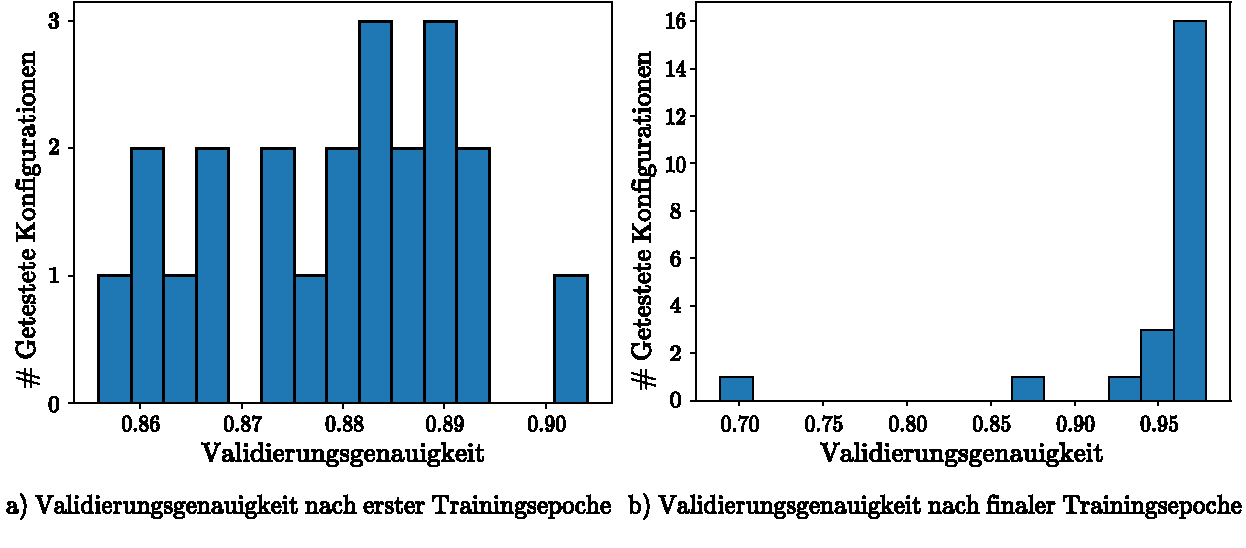
\includegraphics[scale=0.750]{NNOPT/init_and_end_perf_finetuning.pdf}
\caption{Erreichte Klassifikationsgenaugikeit nach der ersten bzw. letzten Epoche des Fine-Tunings, der getesteten Konfigurationen}
\label{finetuning_int_end}
\end{figure}
\\
Betrachtet man die Ergebnisse der Testläufe in Kombination mit den dazugehörigen Hyperparametern (siehe Abb.\ref{finetuning_all}), so scheint die Anzahl an Trainingsepochen keinen signifikanten Einfluss auf die erzielte Validierungsgenauigkeit zu haben. Dies deckt sich mit der Annahme, dass sich Netzwerkparameter mittles Fine-Tuning in wenigen Epochen optimieren lassen. Betrachtet man den Trainingsverlauf des Fine-Tunings (vgl. Abb. \ref{finetuning_lr_gamma_verlauf}), so stellt man fest, das für die meisten Konfigurationen nach $10-15$ Epochen keine großen Verbesserungen mehr im Hinblick auf die Validierungsgenauigkeit erzielt werden.  
\begin{figure}[h]
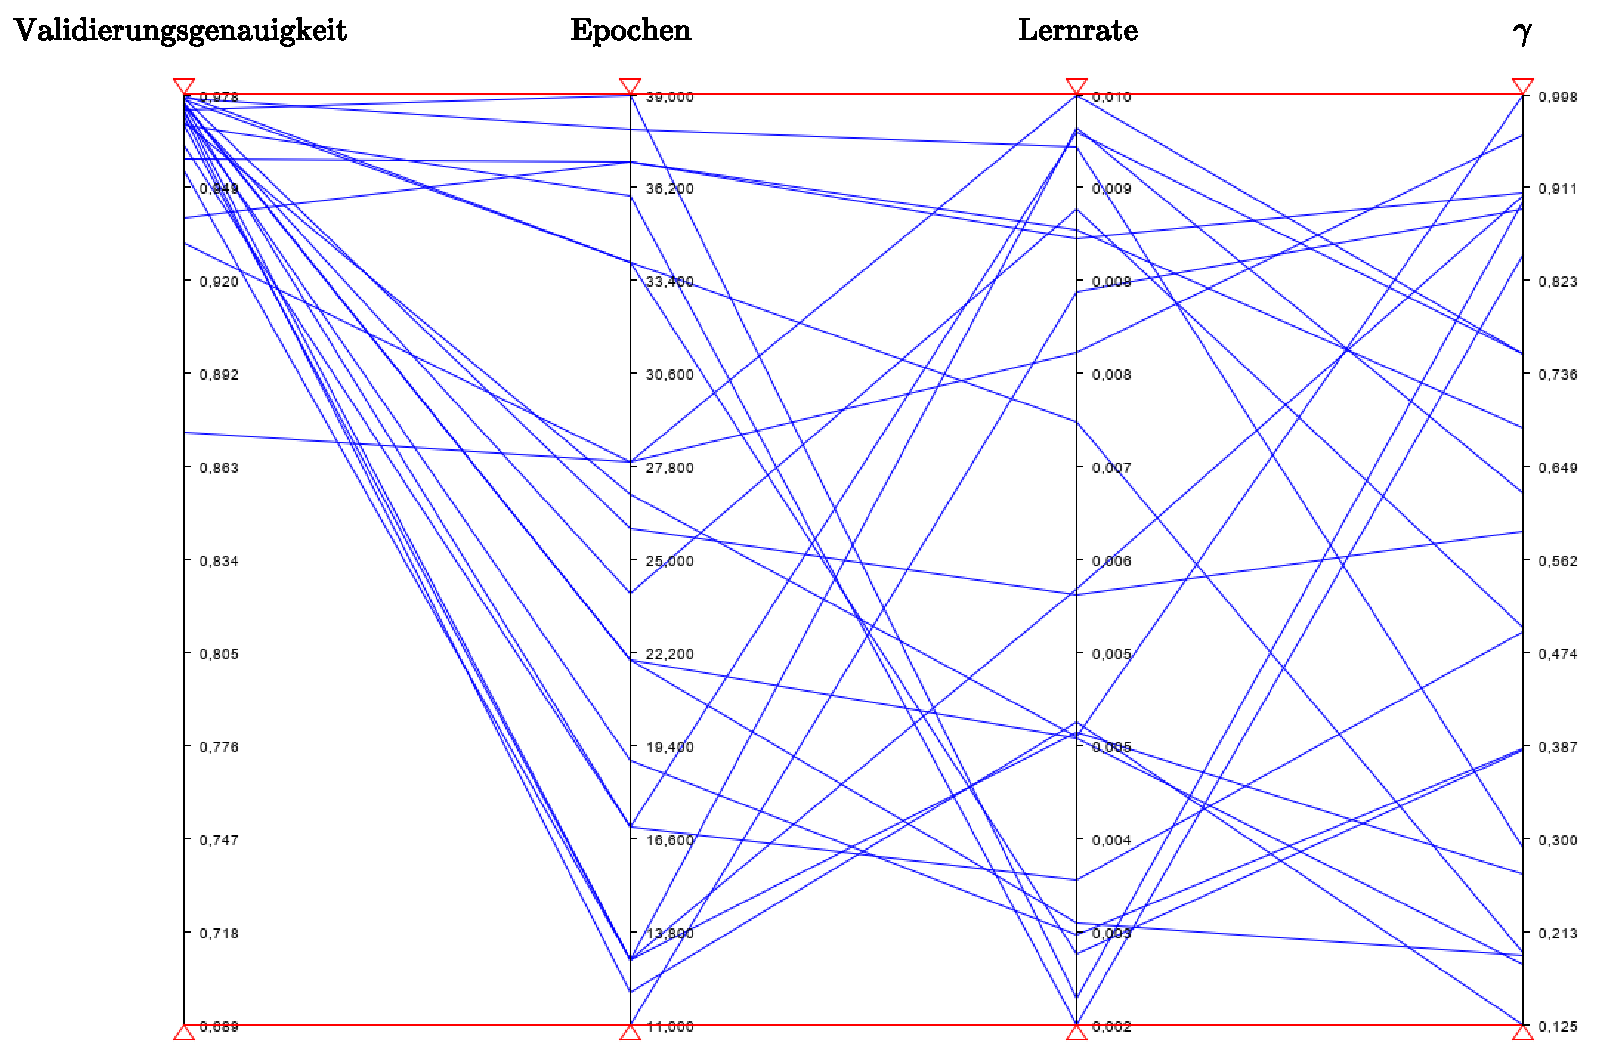
\includegraphics[scale=0.58]{NNOPT/finetuning_all.pdf}
\caption{Parallele Darstellung der getesteten Konfigurationen des Fine-Tunings. Jede Linie repräsentiert einen Konfiguration und die von ihr erzielte Validierungsgenauigkeit.}
\label{finetuning_all}
\end{figure}
\\
Beleuchtet man die in den getesteten Konfigurationen genutzten Lernraten, so stellt sich heraus, dass alle Testläufe mit einer Lernrate unter $0.005$ eine sehr gute Validierungsgenauigkeit erreichen. Werden höhere Lernraten genutzt, so unterscheiden sich die erzielten Ergebnisse deutlich stärker. Bezieht man die dazugehörigen $\gamma$-Faktoren mit ein, sieht man, dass Konfigurationen mit hoher Lernrate, aber niedrigem $\gamma$-Faktor, also mit starker Reduktion der Lernrate während des Trainingsverlaufes, ebenfalls sehr gute Ergebnisse erzielen. Läufe mit hoher Lernrate, sowie hohem $\gamma$-Faktor schneiden dagegen eher schlechter ab (Siehe Abb. \ref{finetuning_lr_gamma}). Analysiert man die Trainingsverläufe der unterschiedlichen Konfigurationen (Siehe Abb.\ref{finetuning_lr_gamma_verlauf}), findet sich eine mögliche Erklärung für diese Verhalten. Bei niedriger Lernrate nähert sich die Validierungsgenauigkeit ohne starke Einbrüche einem Maximum an. Ist die Lernrate hoch fluktuiert die Validierungsgenauigkeit jedoch stark. Dies weist darauf hin, dass die Modelle nicht in der Lage sind ein stabiles Optimum für ihre Parameter zu finden. Hohe Lernraten können dazu führen, dass Parameter bei Optimierungsschritten zu stark verändert werden und so ihr Optimum immer wieder überspringen. Nach Abschluss der ersten $10$ Epochen wird die Lernrate mit dem $\gamma$-Faktor multipliziert. Für Läufe mit hoher initialer Lernrate und niedrigem $\gamma$-Faktor lässt ab diesem Punkt ein gleichmäßigerer Lernprozess beobachten. 
\begin{figure}[h]
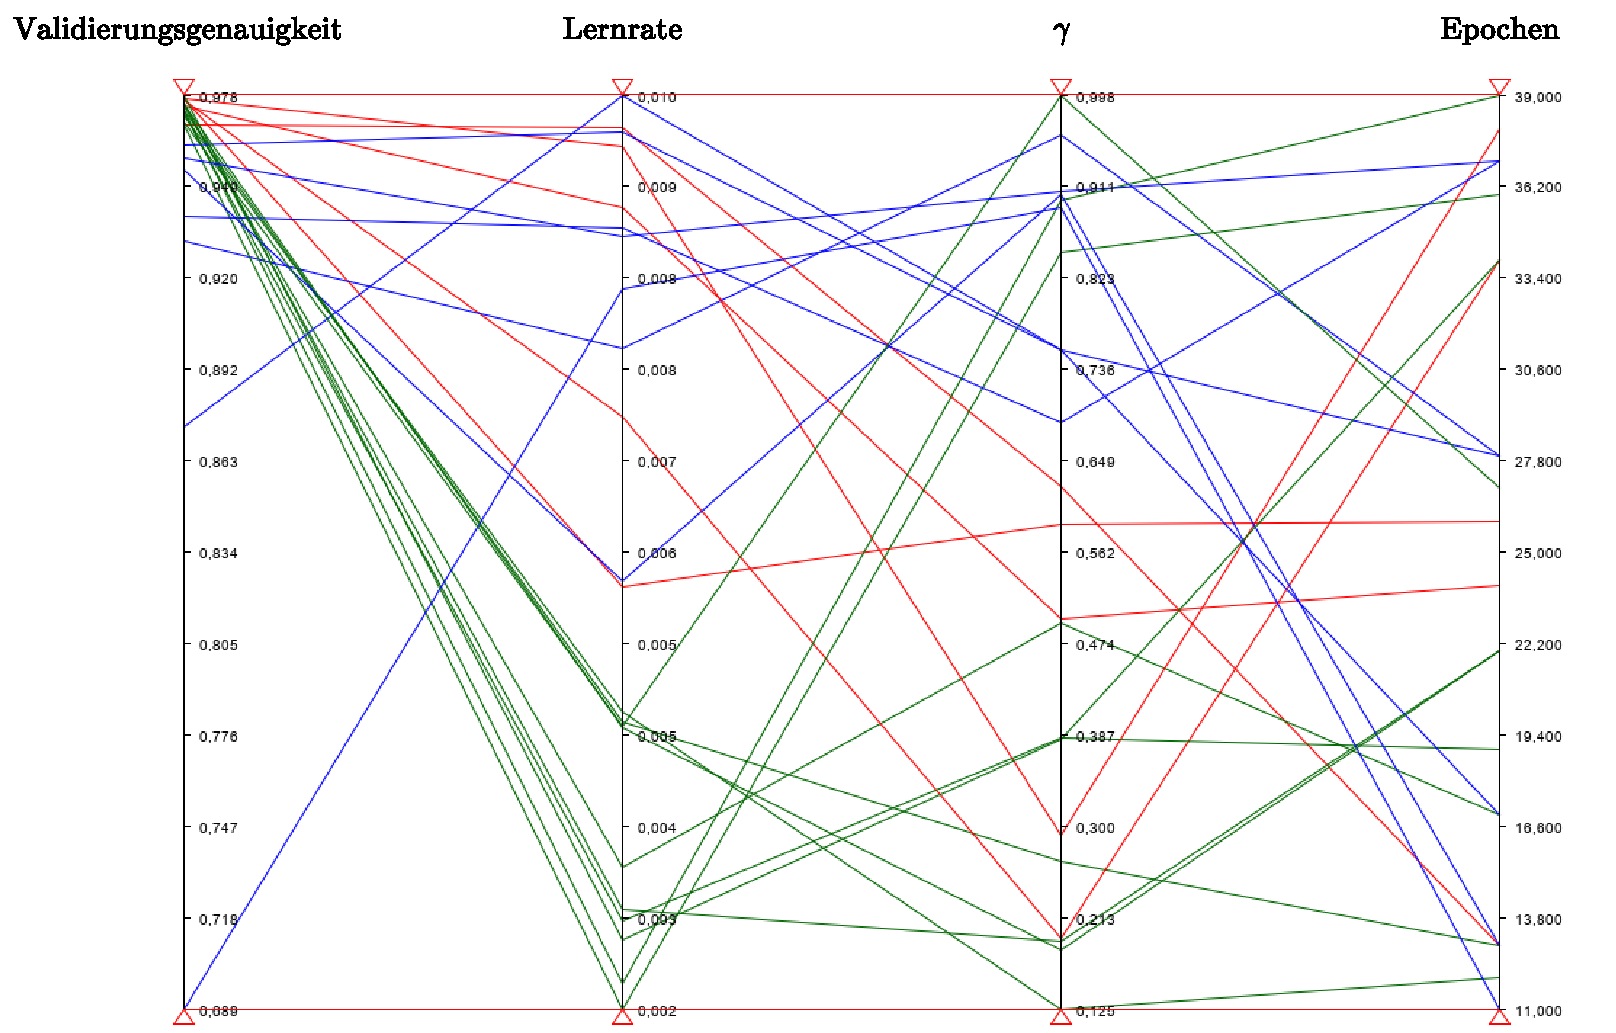
\includegraphics[scale=0.58]{NNOPT/finetuning_lr_gamma.pdf}
\caption{Betrachtung der genutzten Lernraten und $\gamma$-Faktoren. Grün: Konfigurationen mit niedriger Lernrate $(<0.005)$, Rot: Hohe Lernrate und niedriges $\gamma$ $(<0.65)$, Blau: Hohe Lernrate und hohes $\gamma$}
\label{finetuning_lr_gamma}

\centering
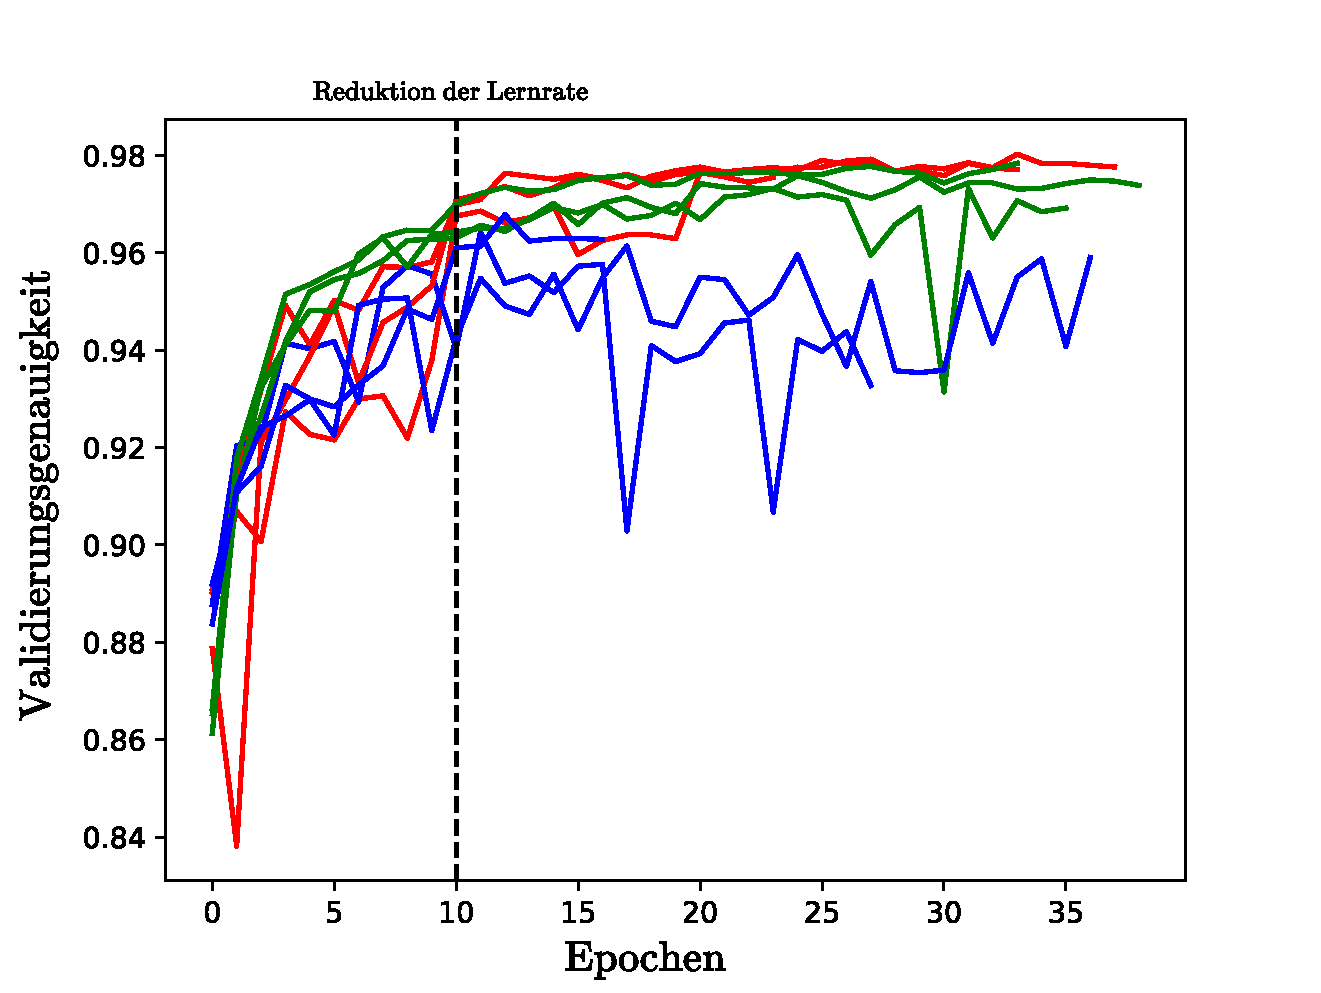
\includegraphics[scale=0.6]{NNOPT/finetuning_lr_gamma_verlauf.pdf}
\caption{Trainingsverlauf der Fine-Tunings, bei unterschiedlicher Lernrate und $\gamma$. Farbgebung analog zu Abb.\ref{finetuning_lr_gamma}}
\label{finetuning_lr_gamma_verlauf}
\end{figure}
\clearpage
Die Konfiguration mit dem besten Trainingsergebnis schreibt eine Trainingsdauer von $22$ Epoche, bei einer initialen Lernrate von $0.0032$ und einem $\gamma$-Faktor von $0.19$ vor und erzielt nach der letzten Epoche eine Validierungsgenauigkeit von $97.6\%$.
\\
Das dabei trainierte Modell ist der Ausgangspunkt für die Hyperparameteroptimierung des Attention-Trainings. Analog wie in den Experimenten zum Fine-Tuning werden mit Hilfe von NNOPT $60$ unterschiedliche Konfigurationen für das Attention-Training getestet. Obwohl das Modell für das Attention-Training durch Entfernung des vierten ResNet-Blocks deutlich verkleinert wird und die Ausgaben des ResNets unter Verwendung des gewichteten Sum-Poolings (vgl. Abb.\ref{attention} auf Seite \pageref{attention}) sehr restriktiv genutzt werden, sind die Attention-Modelle in fast allen untersuchten Konfigurationen in der Lage die Klassifikationsaufgaben weiterhin sehr gut zu Lösen. So werden in $59$ der $60$ untersuchten Konfigurationen eine abschließende Validierungsgenauigkeit von über $89\%$ erreicht (siehe Abb.\ref{attention_int_end}b). Die durchschnittliche Validierungsgenauigkeit nach der letzten Trainingsepoche beträgt $91.3\%$, was einer durchschnittlichen Verschlechterung von $6.3\%$ gegenüber dem verwendeten fine-getunten ResNet-Modell entspricht. Im Kontrast zum Fine-Tuning variiert die gemessene Validierungsgenauigkeit nach der ersten Trainingsepoche der Attention-Trainings deutlich stärker und ist allgemein niedriger (vgl. Abb.\ref{attention_int_end}a). Da die Parameter der zu optimierenden Attention-Einheit nicht vortrainiert sind und daher zufällig initialisiert werden sind größere Unterschiede und schlechter Ergebnisse zu Beginn des Trainings, sowie eine längere benötigte Trainingsdauer zu erwarten.
\begin{figure}[h]
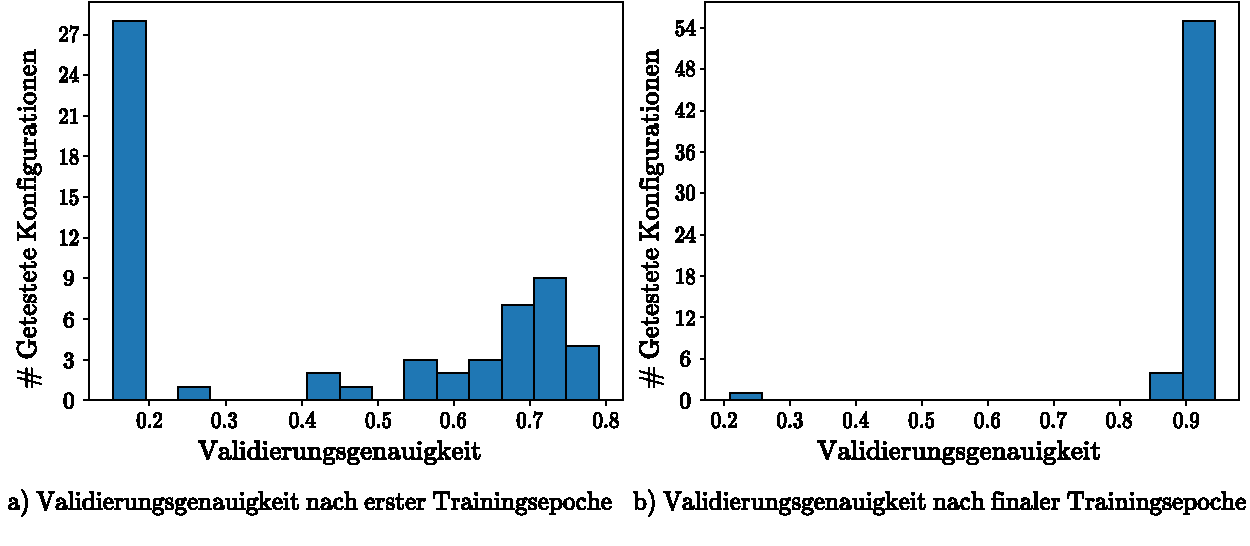
\includegraphics[scale=0.75]{NNOPT/init_and_end_perf_attention.pdf}
\caption{Erreichte Klassifikationsgenaugikeit nach der ersten bzw. letzten Epoche des Attention-Trainings, der getesteten Konfigurationen}
\label{attention_int_end}
\end{figure}
\\
Betrachtet man die genutzte Anzahl an Trainingsepochen in Kombination mit der erreichten Validierungsgenauigkeit(siehe Abb.\ref{attention_epochs}), bestätigt sich diese Annahme. Konfigurationen mit einer Trainingsdauer unter $20$ Epochen erzielen in unseren Experimente durchschnittlich eine geringere Validierungsgenauigkeit. Ab mehr als $20$ Epochen schwächt sich der positive Effekt einer längeren Trainingsdauer jedoch deutlich ab.
\\
\begin{figure}[h]
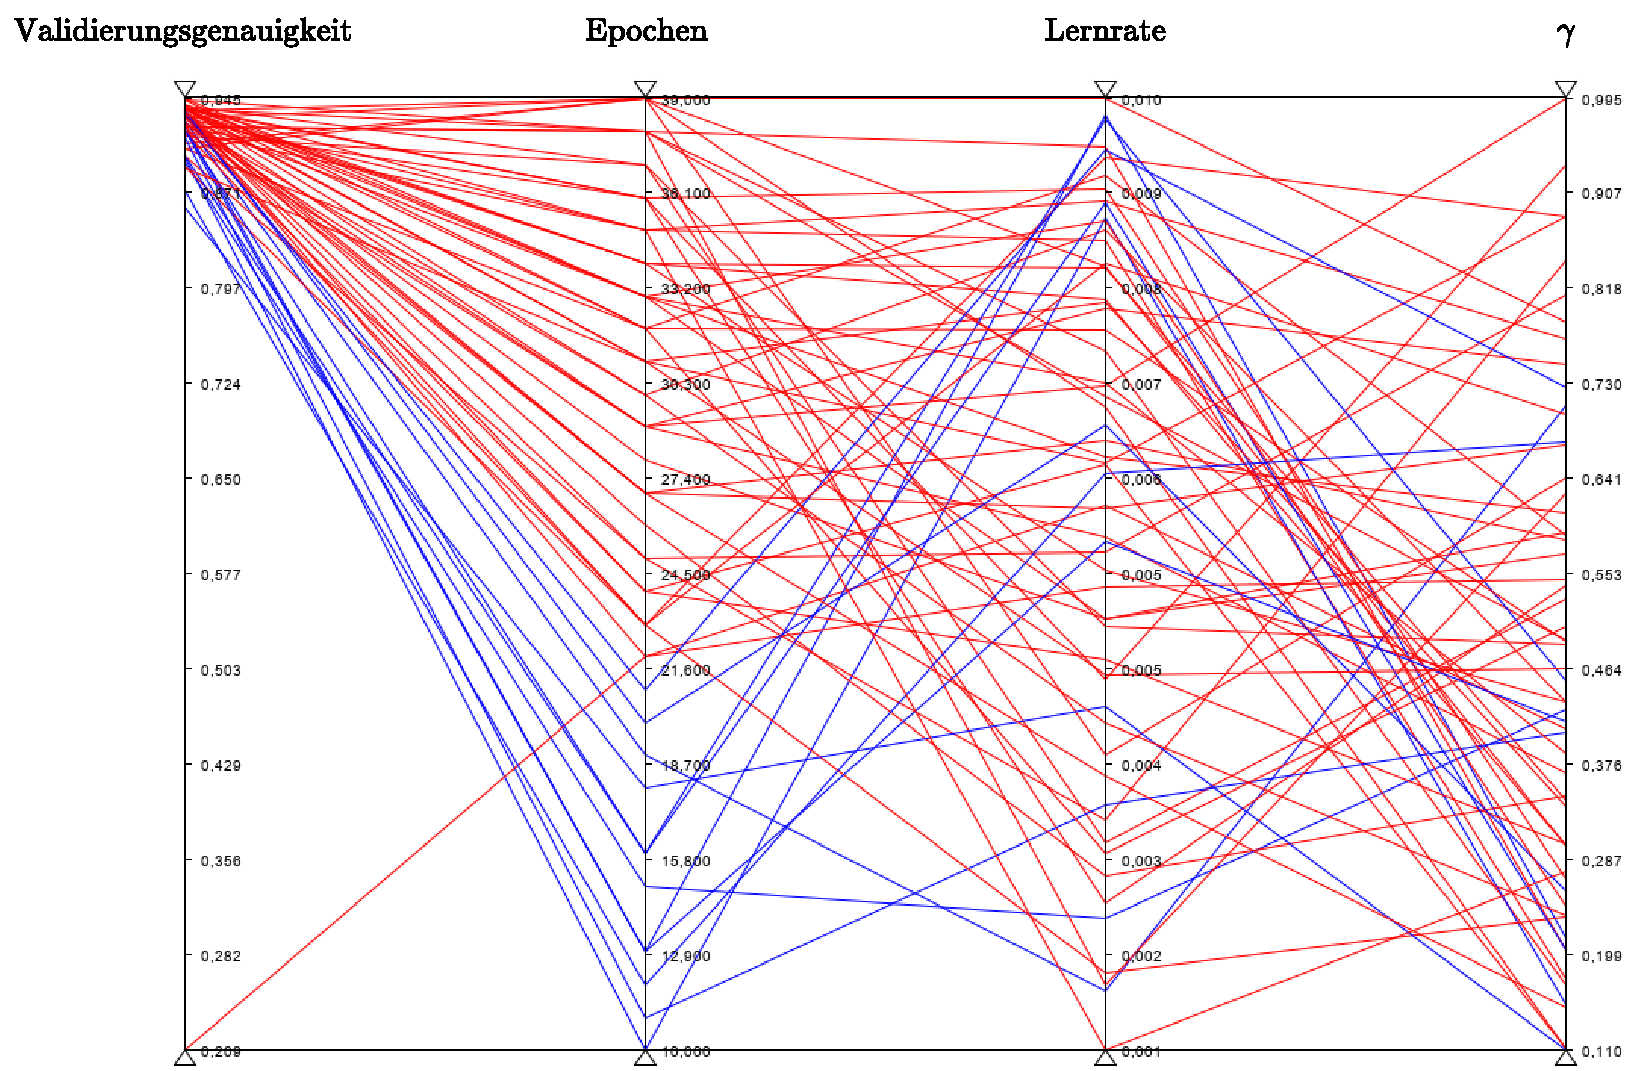
\includegraphics[scale=0.58]{NNOPT/attention_epochs.pdf}
\caption{Betrachtung der gewählten Trainingsdauer. Rot: Über $20$ Epochen, Blau: $20$ oder weniger Epochen}
\label{attention_epochs}
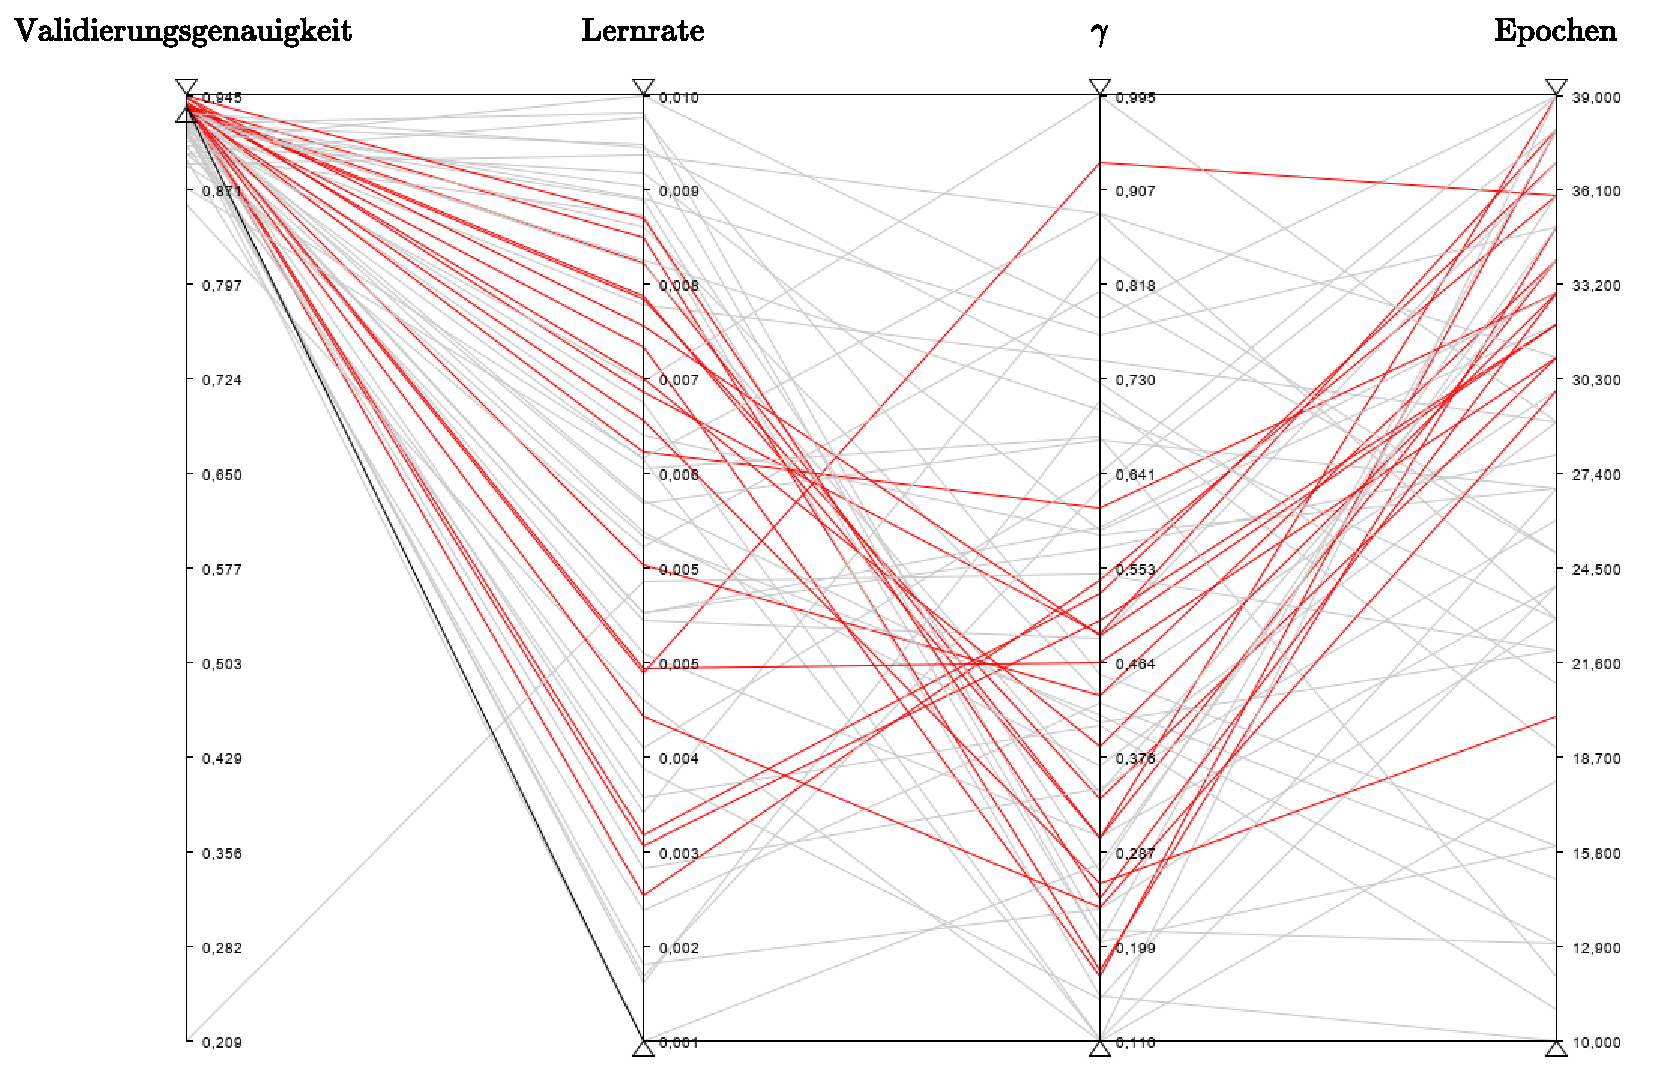
\includegraphics[scale=0.58]{NNOPT/attention_top_runs.pdf}
\caption{Darstellung der Validierungsgenauigkeit nach Trainingsende. Rot: Läufe mit Validierungsgenauigkeit $\geq 93.5\%$, Grau: Läufe mit niedrigerer Validerungsgenauigkeit}
\label{attention_top}
\end{figure}
\clearpage
Für Lernrate und $\gamma$-Faktor lassen sich nur schwer Tendenzen erkennen. Über den gesamten Suchraum dieser Parameter lassen sich sowohl Konfigurationen mit hoher, sowie Konfigurationen mit weniger hoher Validierungsgenauigkeiten erreichen finden. Die Konfigurationen, welche die höchsten Validierungsgenauigkeiten erreichen (Siehe Abb.\ref{attention_top}) nutzen jedoch alle eine Lernrate im Bereich zwischen $0.0025$ und $0.009$. Die $\gamma$-Faktoren dieser Konfigurationen liegen meist unter $0.55$ und die Trainingsdauer über $30$ Epochen.
Die beste gefundene Konfiguration erzielt eine Validierungsgenauigkeit von $94.5\%$ und nutzt dabei eine Lernrate von $0.0078$ einen $\gamma$-Faktor von $0.49$ und eine Trainingslänge von $32$ Epochen. 
Mit Hilfe der ermittelten Hyperparameterwerte der besten gefundenen Konfigurationen für Fine-Tuning und Attention-Training werden $6$ neue Modelle Trainiert, die in den Retrievalexperimenten zur Extraktion der Deskriptoren genutzt werden. Die Trainingsverläufe dieser Modelle sind in Abb.\ref{optimized_runs} dargestellt.
\begin{figure}[h]
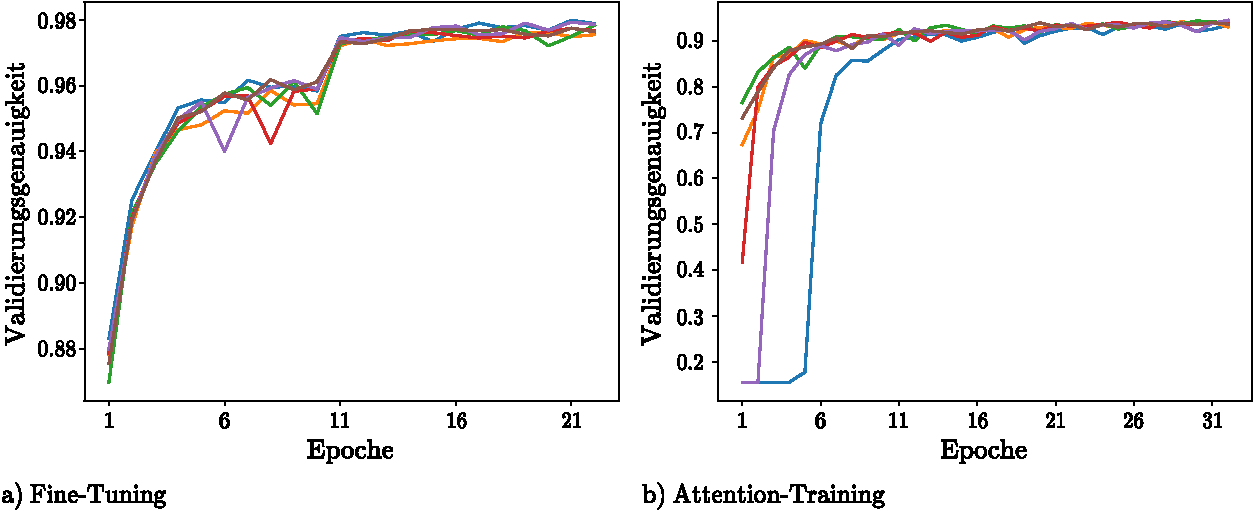
\includegraphics[scale=0.75]{NNOPT/6_model_verlauf}
\caption{Trainingsverläufe mit optimierten Hyperparametern. Gleichefarbige Linen gehören zu gemeinsamen Trainingsläufen.}
\label{optimized_runs}
\end{figure}

\subsection{Variieren der Deskriptorlänge}\label{pca_experiments}

Nach Betrachtung der Trainingsphasen und Erstellung optimierter Modelle, werden nun Parameter aus den späteren Phasen des Verfahrens untersucht.
Ein zentraler Parameter der Extraktions- und Verarbeitungsphase ist die Anzahl an Dimensionen, der Deskriptoren nach der Transformation mittels Hauptkomponentenanalyse (vgl. \ref{pca_chapter} auf Seite \pageref{pca_chapter}). Da die zu einem Suchdatensatz erstellte Repräsentation fast ausschließlich aus den transformierten Deskriptoren besteht, sind diese für den überwiegenden Teil des Speicherbedarfs verantwortlich, der während der aktiven Verwendung des Suchsystems anfällt \footnote{Bei der Suche nach den ähnlichsten Deskriptoren während dem Matching hat die Deskriptorlänge auch einen Einfluss auf die Laufzeit. Da der Rechenaufwand für die geometrische Verifizierung von Matches, die nicht von der Deskriptorlänge abhängt, jedoch deutlich größer ist, ist dieser Einfluss vernachlässigbar.}. Insbesondere bei der Suche in großen Datenbanken ist es daher notwendig die Deskriptoren stark zu komprimieren. Durch die verwendete Art der Komprimierung geht jedoch auch immer ein Teil der ursprünglich in den Deskriptoren enthaltenen Informationen verloren. Es wird erwartet, dass sich der Informationsverlust durch die Deskriptortransformation negativ auf die Qualität des initialen Deskriptormatchings auswirkt. Um diesen Informationsverlust zu quantifizieren wird der Anteil der ursprünglichen Varianz zwischen den Deskriptoren errechnet, die nach der Transformation erhalten bleibt. Hierbei werden alle Deskriptoren betrachtet, die für die Berechnung der Hauptkomponentenanalyse genutzt wurden. Es ist davon auszugehen, dass sich der Informationsverlust auf unbeteiligten Deskriptoren ähnlich verhält. Die Autoren des DELF-Papiers \cite{delf} schlagen als Kompromiss zwischen erhaltener Information und Kompaktheit vor die Deskriptoren auf $40$ Dimensionen zu reduzieren. Wie dieser Wert ermittelt wurde wird jedoch nicht beschrieben. Um eine geeigneten Anzahl an Dimensionen zu ermitteln werden neben der von den Autoren empfohlenen Anzahl auch die Hälfte bzw. ein Vielfaches an erhaltenen Dimensionen, bis zu $200$ getestet. In Abb. \ref{explained_variance_ratio} wird der Einfluss der Deskriptorlänge auf den Anteil der erklärten ursprünglichen Varianz dargestellt.
\begin{figure}[h]
\centering
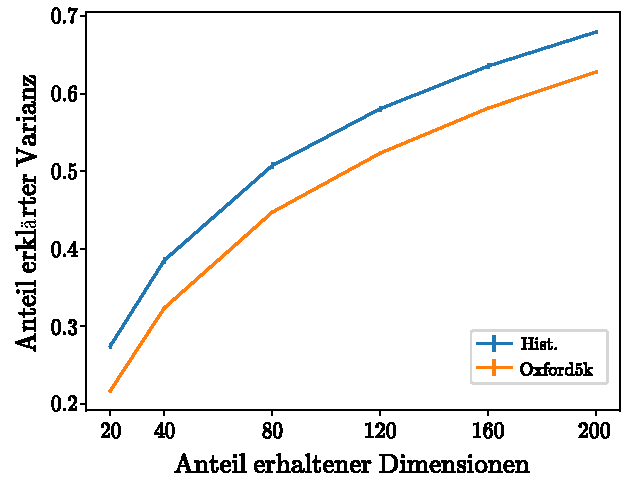
\includegraphics[scale=1]{explained_variance.pdf}
\caption{Erklärter Anteil der Varianz nach Deskriptortransformtion durch Hauptkomponentenanalyse auf unterschiedlichen Retrievaldatensätzen, je nach Anzahl erhaltener Dimensionen.}
\label{explained_variance_ratio}
\end{figure}
Die Variation der Deskriptorlänge hat nicht nur Einfluss darauf, welche Deskriptorpaare während dem initialen Matching bestimmt werden, sondern auch wie groß die euklidische Distanz zwischen diesen Paaren ist. Die Deskriptoren werden vor dem Matching zwar Längennormiert, sodass der maximale Abstand zwischen Deskriptoren $2$ beträgt. Der mittlere Abstand der bestimmten Deskriptorenpaare ist jedoch von der Varianz zwischen den Deskriptoren abhängig und steigt daher mit wachsender Deskriptorlänge. Während dem initialen Deskriptormatching werden Matchingpaare, deren Abstand über einem Distanzschwellwert liegen verworfen, um inkorrekte Matches auszusortieren (siehe Alg.\ref{descmatch} auf Seite \pageref{descmatch}). In Abb. \ref{influence_dim} lässt sich beobachten, wie sich die Anzahl an gefundenen Deskriptoren-Matches mit steigender Länge der verwendeten Deskriptoren verringert, wenn der gewählte Distanzschwellwert unverändert bleibt. In Abb. \ref{influence_threshold} ist analog, bei einer konstanten Deskriptorlänge von $80$ der Einfluss von unterschiedlichen Schwellwerten dargestellt. Je größer der Schwellwert, desto weniger Deskriptorenmatches werden aussortiert. Die unterschiedlichen untersuchten Deskriptorenlänge, werden daher auch mit mehreren unterschiedlichen Schwellwerten getestet um geeignete Kombinationen zu finden. 

\begin{figure}[H]
\centering
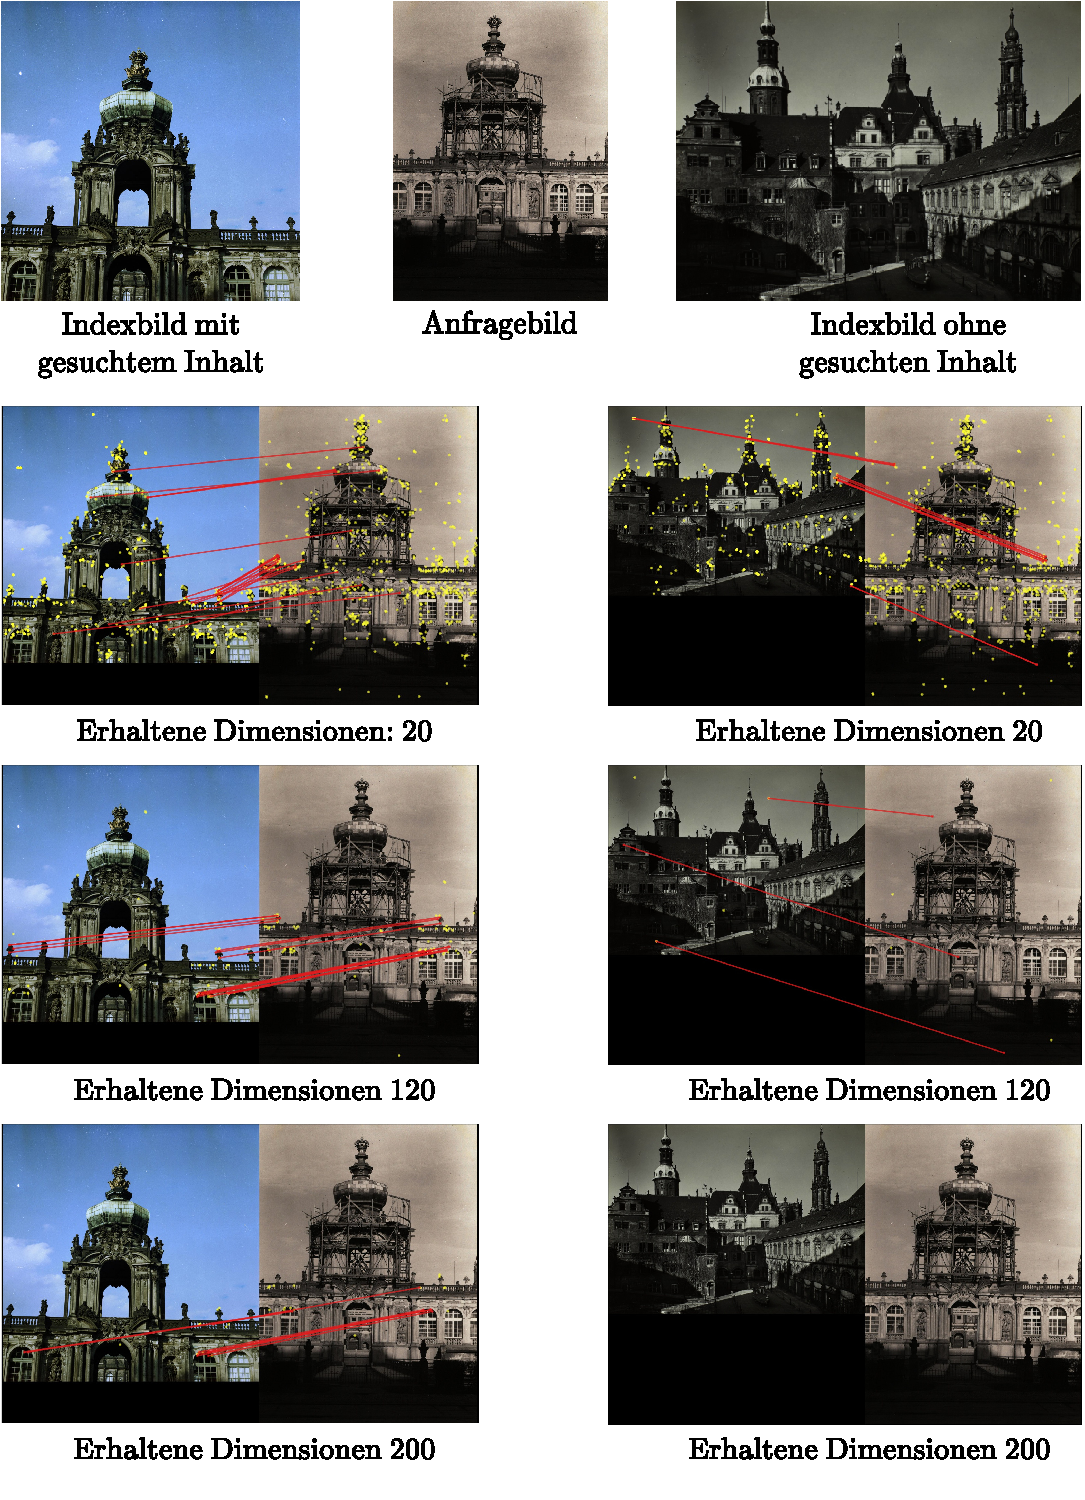
\includegraphics[scale=0.86]{influence_dim}
\caption{Einfluss der Deskriptorlänge auf das Deskriptorenmatching zwischen Anfragebild und Bildern mit und ohne gesuchtem Bildinhalt aus dem Suchindex, bei einem Schwellwert für maximale Deskriptordistanz von $0.8$. Gelbe Punkte markieren Deskriptoren die im Partnerbild gematched wurden. Rote Linien markieren geometrische verifizierte Matches}
\label{influence_dim}
\end{figure}

\begin{figure}[H]
\centering
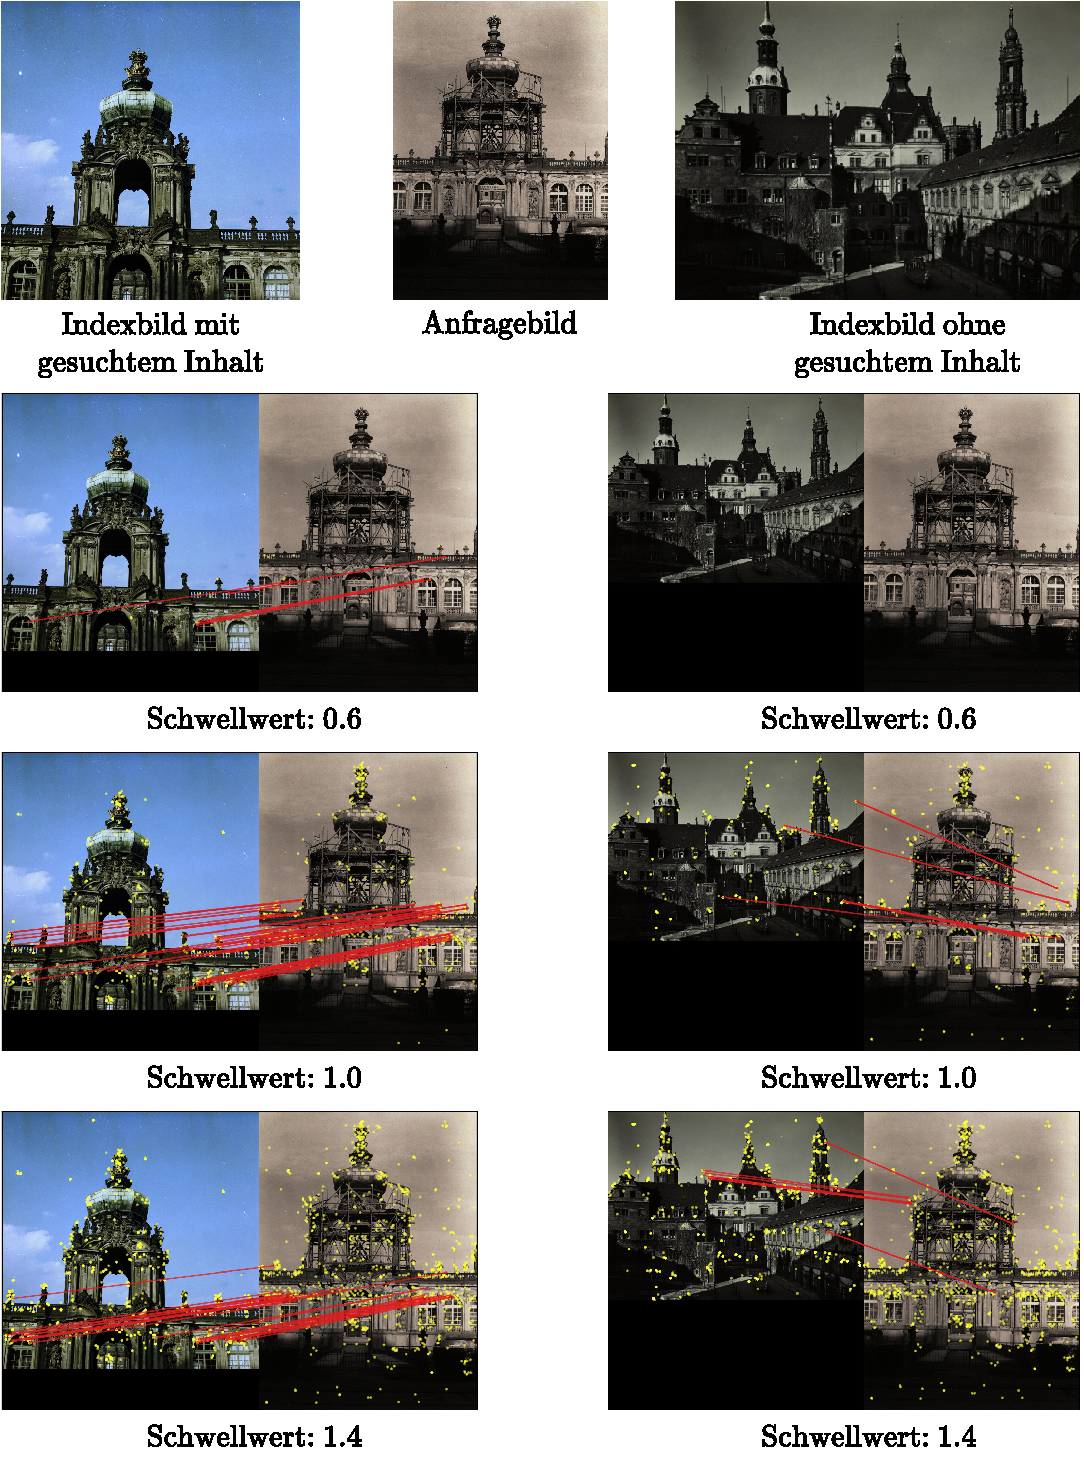
\includegraphics[scale=0.86]{influence_threshold}
\caption{Einfluss des Distanzschwellwerts auf das Deskriptorenmatching, bei Verwendung von $80$ dimensionalen Deskriptoren. Gelbe Punkte markieren Deskriptoren die im Partnerbild gematched wurden. Rote Linien markieren geometrische verifizierte Matches}
\label{influence_threshold}
\end{figure}

Die Autoren der DELF-Papiers \cite{delf} verwenden für $40$-Dimensionale Deskriptoren einen Schwellwert von $0.8$. 
Im Folgenden werden neben diesem Wert sowohl kleiner, wie auch größere Werte zwischen $0.6$ und $1.4$ in Intervallschritten von $0.2$ getestet. Alle Parameterkombinationen von Deskriptorlänge und Distanzschwellwert werden auf den $6$ trainierten Modellen getestet. Für die Auswertung werden die Ergebnisse jeweils über die Läufe der $6$ Modelle gemittelt. Zusätzlich werden Fehlerbereiche im Größer der Standardabweichung angegeben. In Abb. \ref{mAP_num_dim} ist für alle betrachteten Konfigurationen von Deskriptorlänge und Distanzschwellwert, die auf dem historischen Datensatz sowie auf den Oxford5k-Daten getestet werden, die erreichte mAP dargestellt.

\begin{figure}[h]
\includegraphics[scale=0.74]{mAp_num_dim}
\caption{Erreichte mAP bei unterschiedlicher Deskriptorlänge und Distanzschwellwert.}
\label{mAP_num_dim}
\end{figure}

\begin{figure}[h]
\includegraphics[scale=0.74]{mAp_var_dist_ratio}
\caption{Erreichte mAP bei unterschiedlichen Verhältnissen zwischen erklärtem Varianzanteil und gewähltem Distanzschwellwert.}
\label{mAP_var_dist_ratio}
\end{figure}
Unabhängig der getesteten Konfiguration erzielt DELF auf dem Oxford5k-Datensatz eine deutlich höhere mAP als auf den historischen Daten. Welche Aspekte des historischen Datensatzes für das DELF-Verfahren besonders schwierig sind wird anschließend an die Parameterbetrachtung genauer betrachtet. Wie erwartet lassen sich mit größerer Deskriptorlänge bei geeignetem Distanzschwellwert tendenziell bessere Ergebnisse erzielen. Die beste gefundene Konfiguration auf den historischen Daten nutzt Deskriptoren der Länge $160$ bei einem Schwellwert von $1.0$ und erzielt im Mittel eine mAP von $0.57$. Auf Oxford5k erreicht die beste Konfiguration im Mittel eine mAP von $0.71$ und nutzt dabei eine Deskriptorlänge von $120$, mit einen Schwellwert von $1.0$ . Allerdings lässt sich auf Oxford5k mit der von den DELF-Autoren empfohlenen Deskriptorlänge von $40$ und dem empfohlenen Schwellwert von $0.8$ mit einer mittleren mAP von $0.70$ bereits fast gleich gute Ergebnisse erzielen. Lediglich bei Verwendung von noch kleineren Deskriptoren lassen sich signifikante Performanzeinbußen feststellen. So erreicht die beste Konfiguration mit Deskriptorlänge $20$ im Mittel nur eine mAP von $0.65$. Auf den historischen Daten lassen sich mit Deskriptoren mit mehr als $40$ Dimensionen noch signifikante Verbesserungen erzielen. So erreicht die beste Konfiguration mit $80$ Dimensionen eine im Mittel um $0.03$ höhere mAP als die von den Autoren empfohlene Konfiguration. Eine weitere Vergrößerung der Deskriptoren ziehen allerdings auch auf den historischen Daten keine großen Performanzverbesserungen nach sich.
\\
Bei Betrachtung der Distanzschwellwerte, stellt man fest, dass der optimale Schwellwert mit der Länge der verwendeten Deskriptoren steigt. Dies deckt sich mit den Beobachtungen aus Abb. \ref{influence_dim} und Abb. \ref{influence_threshold}, da mit wachsender Deskriptorlänge ein höherer Schwellwert gewählt werden muss, um eine adäquate Anzahl an Deskriptormatches zu erhalten. Bei einem zu klein gewählten Schwellwert werden fast alle potentiellen Deskriptormatches aussortiert, was zu einem drastischen Perfomanzverlust führt. Ein zu groß gewählter Schwellwert führt ebenfalls zu Performanzverlusten, welche jedoch deutlich geringer ausfallen. Das ist der zusätzlichen geometrischen Verifikation mittels RANSAC zu verdanken. Selbst wenn durch den Schwellwert keine unerwünschten Deskriptormatches verworfen werden, wird ein Großteil dieser Matches während der geometrischen Verifikation durch keine Transformation erklärt und so aussortiert\footnote{In Abb. \ref{feature_score_map} auf Seite \pageref{feature_score_map} wird deutlich, dass die Performanz stark unter einem zu hohen Schwellwert leidet, wenn keine geometrische Verifikation durchgeführt wird.}. \\
Wie bereits erläutert hängt die Wahl eines geeigneten Schwellwerts stark von der Länge der Deskriptoren bzw. dem Anteil der von ihnen erklärten Varianz ab. Ein mögliche Strategie für die Untersuchung von vielen unterschiedlichen Deskriptorlänge ist daher den Schwellwert direkt abhängig von der erklärten Varianz zu bestimmen und so die Anzahl zu testender Konfigurationen zu reduzieren. In Abb. \ref{mAP_var_dist_ratio} ist die erreichte mAP im Bezug zum Verhältnis zwischen erklärter Varianz und Schwellwert abgebildet. Tatsächlich erreichen fast alle Deskriptorlängen ihr bestes Ergebnis, wenn das Verhältnis zwischen dem Anteil der erklärten Varianz und dem gewählten Schwellwert zwischen $0.5$ und $0.7$ liegt. Für die Untersuchung anderer Deskriptorlängen wäre es daher sinnvoll Schwellwerte zu testen, die innerhalb dieses Bereiches liegen.



\chapter{Fazit und Ausblick}

Ziel der vorliegenden Arbeit ist es zu untersuchen, ob das Image Retrieval System DELF für die inhaltsbasierte Suche auf historischen Daten geeignet ist und welche Stärken und Schwächen es im Vergleich zu alternativen Verfahren aufweist. Weiterhin sollen die Einflüsse unterschiedlicher Parameter innerhalb der DELF-Pipeline analysiert werden, um diese für die Domäne der historischen Aufnahmen zu optimieren.
\section{Fazit}
Es zeigt sich, dass das DELF-Verfahren bei der Anwendung auf historischen Aufnahmen nicht nur eine deutliche Verbesserung gegenüber einer zufälligen Suche darstellt, sondern in den meisten betrachteten Bilderkategorien auch signifikant bessere Ergebnisse als das im Vergleich betrachtete ConvNet-Verfahren erzielt. Trotz des relativ hohen Rechenaufwands, der insbesondere durch den zusätzlichen Schritt der geometrischen Verifikation entsteht, ist DELF damit aktuell ein vielversprechendes Verfahren für den Einsatz im HistStadt4D-Projekt.
\\
Eine Stärke des DELF-Verfahrens ist sein Umgang mit Luftaufnahmen, welche einen besonders schwierigen Aspekt des historischen Datensatzes bilden. So erzielt das DELF-Verfahren in Kategorien, die häufig in Luftaufnahmen zu finden sind, besonders deutliche Verbesserungen gegenüber dem ConvNet-Verfahren. 
\\
Als problematisch hat sich für das DELF-Verfahren der Umgang mit schlecht belichteten bzw. Nachtaufnahmen erwiesen. So ist DELF kaum in der Lage, gleiche Bildinhalte, bei sehr unterschiedlichen Belichtungsverhältnissen zu erkennen. Das ConvNet-Verfahren scheint hingegen kaum von dieser Problematik betroffen zu sein.
\\
Sowohl das DELF- als auch das ConvNet-Verfahren können in Aufnahmen aus unterschiedlichen zeitlichen Perioden, in denen sich die betrachteten Objekte durch Umbauten oder Zerstörung stark voneinander unterscheiden, kaum gemeinsame Bildinhalte feststellen. Aktuell sind uns keine Möglichkeiten bekannt, mit solchen Veränderungen effektiv umzugehen.
\\
Objekte, die eine Vielzahl von sich ähnelnden Elementen wie Fenster oder Torbögen enthalten, sind für DELF, insbesondere wegen des geometrische Verifikationsschritts mittels RANSAC, problematisch. Diese sich wiederholenden Bildinhalte werden aufgrund ihrer Ähnlichkeit zueinander oft falschen Instanzen in dem betrachteten Vergleichsbildern zugeordnet, was zu geometrisch nicht erklärbaren Korres\-pondenzen führt. In der Parameteranalyse hat sich gezeigt, dass diese Problematik auf dem historischen Datensatz so ausgeprägt ist, dass das DELF-Verfahren hier ohne geometrische Verifikation gleich gute Ergebnisse erzielt. Die Vergleichsanalyse auf dem Benchmark-Datensatz Oxford5k zeigt sogleich, dass sich mittels RANSAC bei der Betrachtung von Objekten mit weniger Wiederholungen eine signifikante Verbesserung der Retrievalperformanz erreichen lässt. 
\\
Die Analyse unterschiedlicher Extraktionspunkte für die Erstellung von Deskriptoren hat ergeben, dass sich die letzten Schichten des ResNets nicht für die Extraktion von DELF-Deskriptoren eignen. Insbesondere das zur Selektion der Deskriptoren trainierte Attention-Netzwerk hat Schwierigkeiten, geeignete Deskriptoren auszuwählen, wenn es auf den Ausgaben des letzten ResNet-Blocks trainiert wurde. Bei einer Extraktion aus dem vorletzten ResNet-Block, wie von den DELF-Autoren empfohlen, werden deutlich bessere Retrievalergebnisse erzielt.
\\
Ein weiterer betrachteter Parameter ist die verwendete Deskriptorlänge. Dabei zeigt sich, dass durch die Erstellung längerer Deskriptoren geringfügige Verbesserungen der Retrievalperformanz erzielt werden können. Dieser Effekt schwächt sich mit wachsender Länge der Deskriptoren deutlich ab. Zusätzlich steigt der benötigte Speicher- und Rechenbedarf mit der Länge der Deskriptoren an. Für einen geeigneten Kompromiss zwischen Retrievalperformanz und Speicherbedarf bietet sich je nach verwendetem Datensatz eine Deskriptorlänge zwischen $40$ und $80$ Dimensionen an.
\\
Die zu Beginn durchgeführte Hyperparameteranalyse zur Optimierung der beiden Trainingsphasen des DELF-Verfahrens hat ergeben, dass die hier untersuchten Parameter in einem relativ großen Spektrum gewählt werden können, ohne die Trainingsergebnisse stark zu beeinflussen. Unter fast allen getesteten Konfigurationen sowohl im Fine-Tuning als auch im Attention-Training, konnte das DELF-Netzwerk die gestellte Klassifikationsaufgabe mit sehr hoher Genauigkeit lösen. Es ist möglich, dass der relativ kleine verwendete Trainingsdatensatz bestehend aus nur knapp vierzigtausend Bildern keine ausreichende Herausforderung für die genutzte Modellarchitektur darstellt, um größere Unterschiede der Trainingsperformanz aufgrund der Trainingsparameter aufzuzeigen.

\section{Ausblick}
Da DELF unter den aktuell untersuchten Retrivalverfahren die besten Ergebnisse auf dem historischen Datensatz erzielt, ist es sinnvoll, auf den Ergebnissen der vorliegenden Arbeit aufzubauen, um das Verfahren weiter für den Anwendungsfall im HistStadt4d-Projekt zu optimieren. Dabei gibt mehrere Bereiche, die sich für eine weitere Betrachtung anbieten.
\\
Eine Erweiterung der historischen Datenbestände ist für alle weiteren Untersuchungen zu Retrievalsystemen hilfreich. Aktuell umfasst der Datensatz nur sieben unterschiedliche Kategorien, die teilweise mit sehr unterschiedlicher Häufigkeit vorkommen. Eine größere Vielfalt an Kategorien kann helfen, weitere Stärken und Schwächen der Verfahren zu erkennen und ermöglicht eine Untersuchung, die einem realistischen Anwendungsfall näher kommt. Eine ausgeglichenere Verteilung der unterschiedlichen Kategorien erleichtert außerdem die Interpretation der Ergebnisse.
\\
Für das DELF-Training wäre auch eine Erweiterung der Trainingsdaten sehr nützlich. Das aktuell verwendete Subset des Google Landmark V2 Datensatzes enthält einen großen Anteil an Gebäudeaufnahmen. Hierbei handelt es sich jedoch nur sehr selten um historische Aufnahmen. Auch Bildinhalte, die sich in den durchgeführten Experimenten als besonders herausfordernd gezeigt haben wie Luft-, Nacht-, oder Aufnahmen von zerstörten Gebäuden finden sich kaum in den verwendeten Trainingsdaten. Das Hinzufügen von historischen Aufnahmen erlaubt es dem DELF-Verfahren möglicherweise besser, mit solchen Inhalten umzugehen. Um geeignete Aufnahmen für einen Trainingssatz zu finden und zu annotieren können große Bilderarchive wie Europeana\footnote{\url{https://www.europeana.eu/de}, zuletzt besucht 21.10.2020} genutzt werden, die eine auf Metadaten basierte Suche auf großen Datenmengen ermöglichen. Mit den aktuell bereits verfügbaren Retrievalsystemen können anschließend gewonnene Suchergebnisse weiter verfeinert bzw. Aufnahmen mit unerwünschten Inhalten aussortiert werden.
\\
Die Aufdeckung der Probleme des DELF-Verfahrens, Deskriptorpaare zwischen sich wiederholenden Bildinhalten geometrisch zu verifizieren, ist eine der zentralen Erkenntnisse, die in der vorliegenden Arbeit gewonnen wurden. Somit stellt die Entwicklung einer Strategie, mit solchen Inhalten sinnvoll umzugehen und dabei weiterhin die Vorteile einer geometrischen Überprüfung zu nutzen, eine wichtige Aufgabe der weiteren Forschungsarbeit zum DELF-Verfahren dar. Ein simpler Ansatz, um diese Problematik zu lösen, wäre es, für Deskriptoren, die große Ähnlichkeiten zu mehreren Deskriptoren in einem betrachteten Vergleichsbild haben, mehrere potentielle Korrespondenzen im RANSAC-Verfahrens zu betrachten. Dadurch steigt die Wahrscheinlichkeit, dass Deskriptorpaare zwischen den korrekten Instanzen sich wiederholender Elemente gefunden werden. 
\\
Im praktischen Einsatz spielt neben Qualität der Suchergebnisse auch die Geschwindigkeit des Suchsystems eine Rolle. Hier besteht aktuell noch viel Raum für weitere Optimierungen. Der für die vorliegende Arbeit erstellte Prototyp des DELF-Verfahrens sammelt viele zusätzliche Informationen, die für die Verfahrensanalyse nützlich sind, die Laufzeit jedoch negativ beeinflussen. Um die Verarbeitung von Suchanfragen zu beschleunigen, ist es sinnvoll, das DELF-Verfahren in einer schnelleren Programmiersprache wie C++ oder JAVA zu implementieren und effiziente Datenstrukturen wie den in Kapitel \ref{pipeline_changes} vorgestellten invertierten Index zu nutzen.

\newpage
\addcontentsline{toc}{chapter}{Anhang}
\pagestyle{empty}
\vspace*{7cm}
\begin{center}
{\Huge Anhang}
\end{center}
\newpage
\pagestyle{fancy}
\markboth{Anhang}{}

\setcounter{figure}{0}
\renewcommand{\thefigure}{\Roman{figure}}


\begin{figure}[h]
\centering
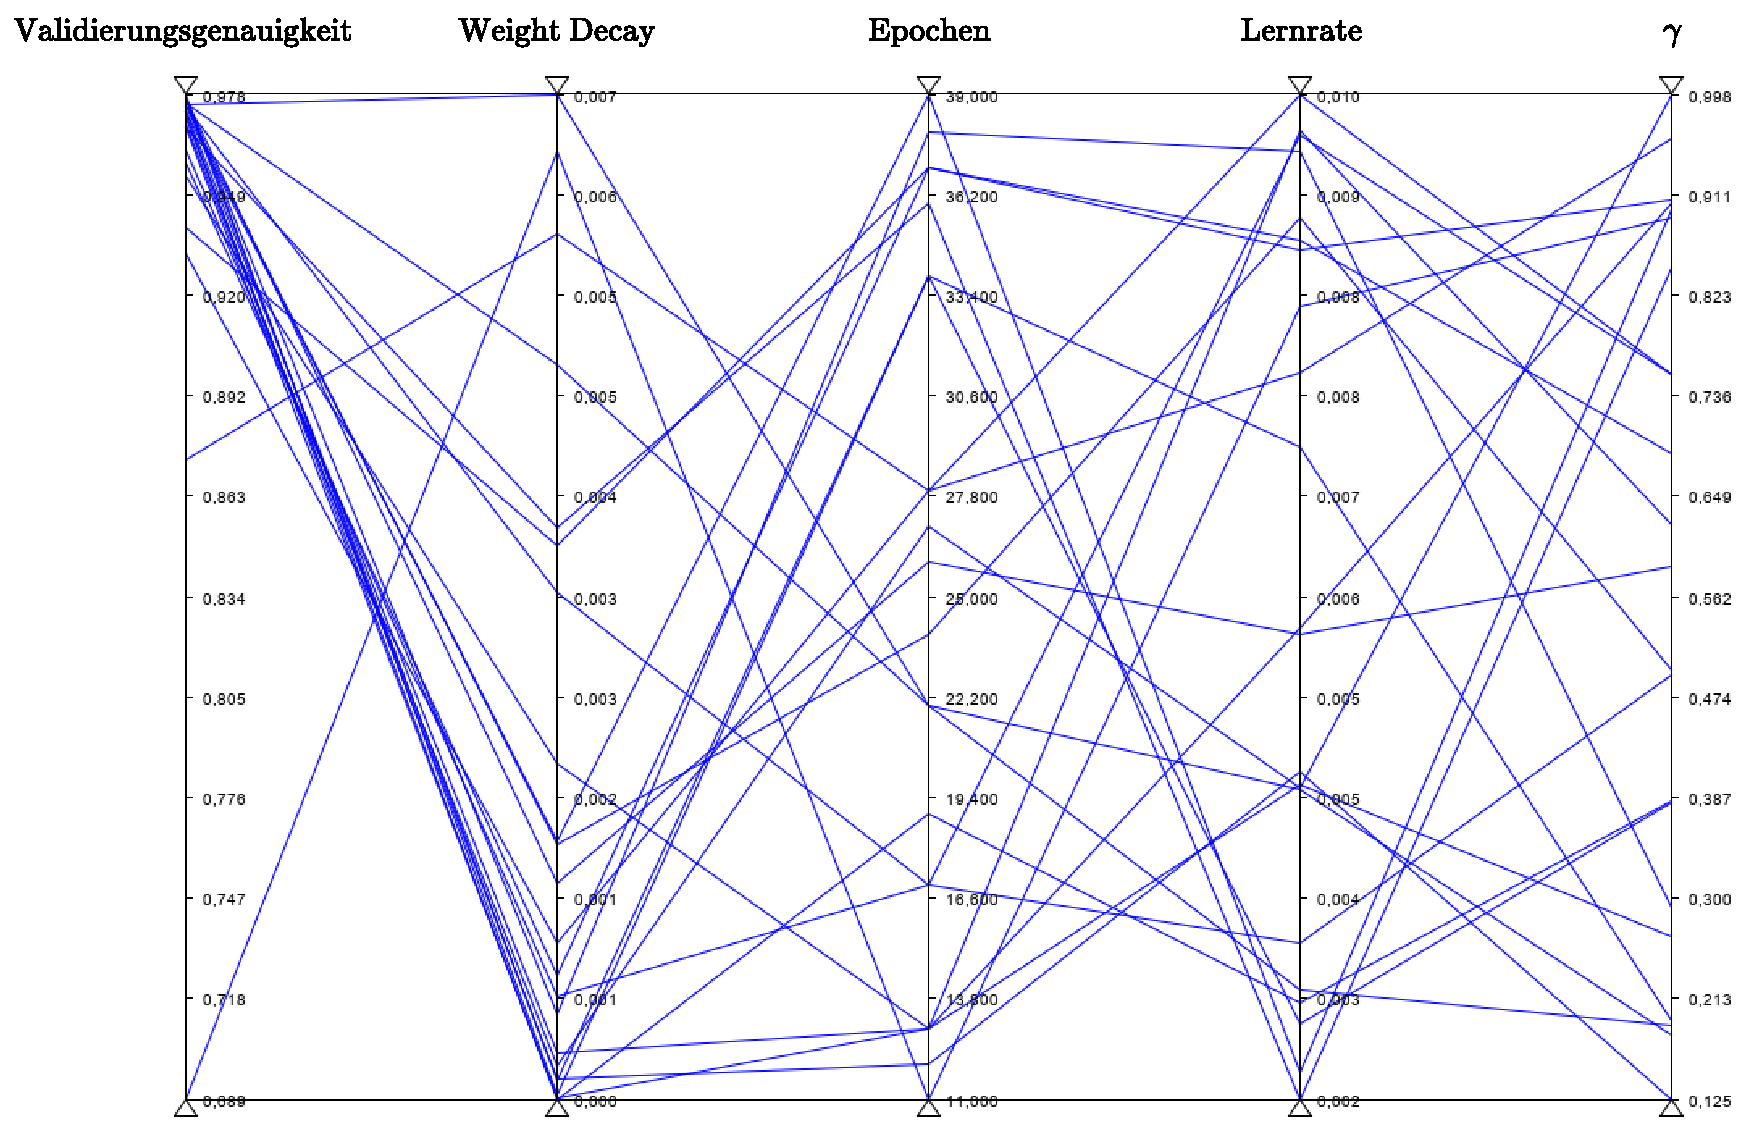
\includegraphics[scale=0.52]{NNOPT/Anhang/layer3_with_weigth_decay_finetuning}
\caption{Ergänzung zu Abb.\ref{finetuning_all} mit zusätzlicher Betrachtung des Weight Decay Parameters. Parallele Darstellung der getesteten Konfigurationen des Fine-Tunings. Jede Linie repräsentiert eine Konfiguration und die von ihr erzielte Validierungsgenauigkeit.}
\label{weight_decay_1}
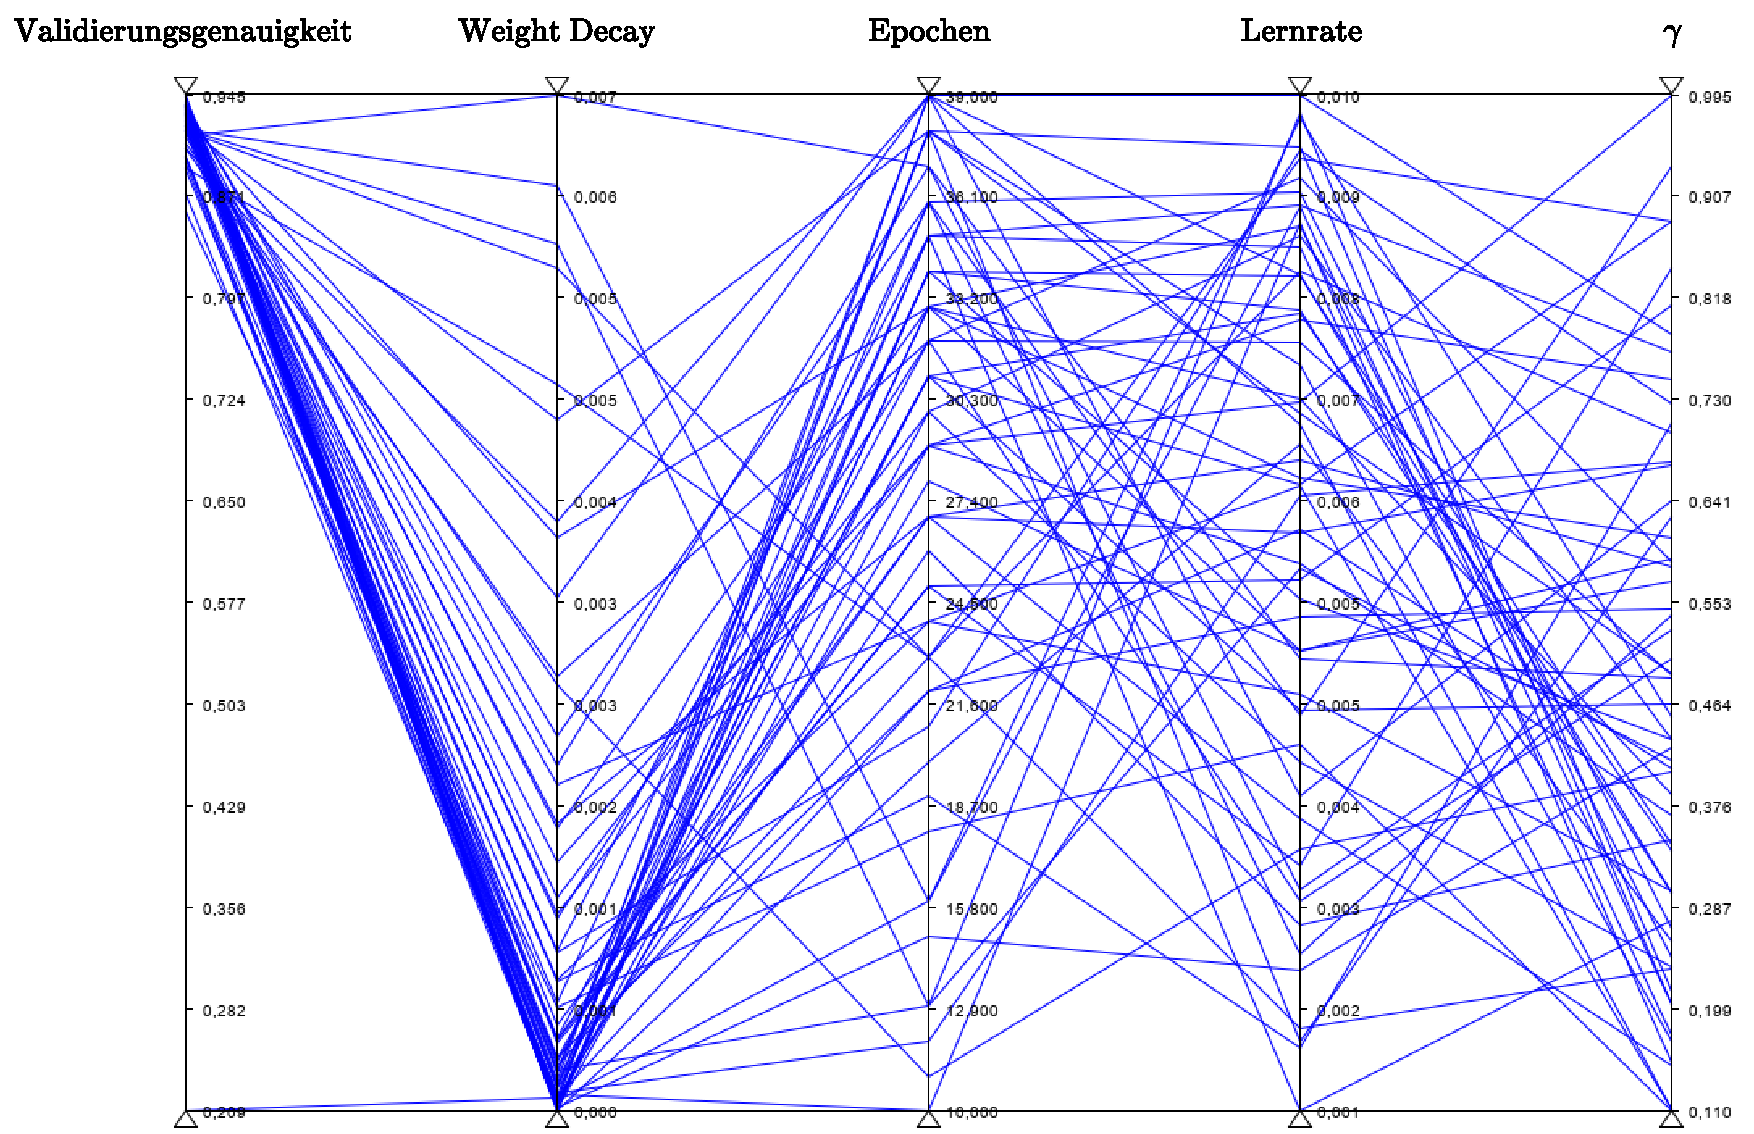
\includegraphics[scale=0.52]{NNOPT/Anhang/layer3_with_weigth_decay_attention}
\caption{Ergänzung zu Abb.\ref{attention_epochs} mit zusätzlicher Betrachtung des Weight Decay Parameters. Parallele Darstellung der getesteten Konfigurationen des Attention-Trainings. Jede Linie repräsentiert eine Konfiguration und die von ihr erzielte Validierungsgenauigkeit.}
\label{weight_decay_2}
\end{figure}

\begin{figure}[h]
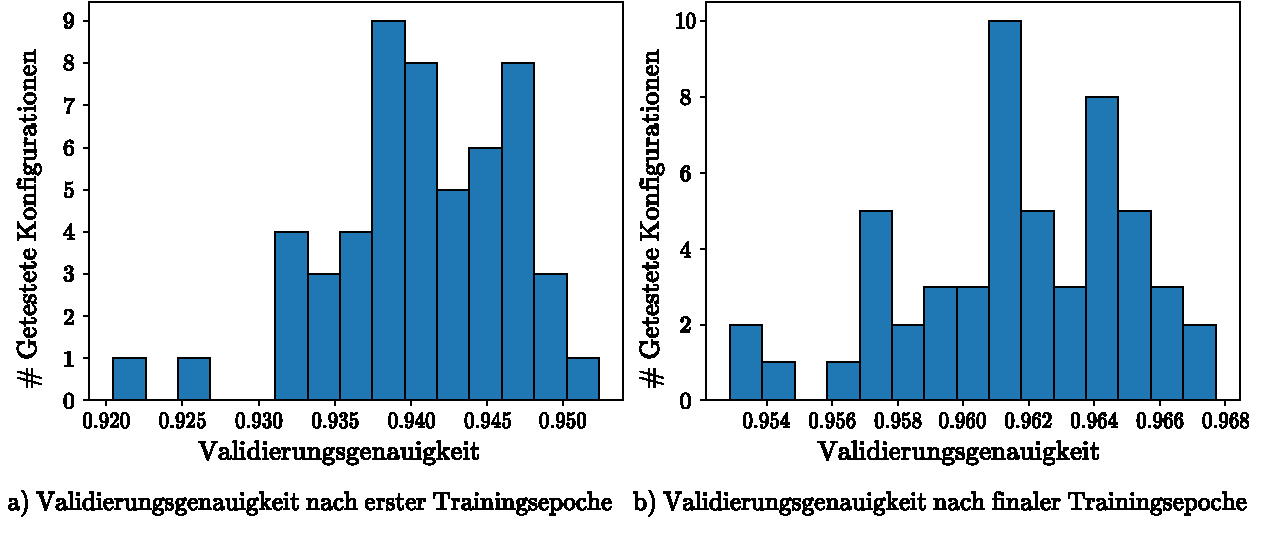
\includegraphics[scale=0.75]{NNOPT/Anhang/layer4_int_and_end_perf_attention.pdf}
\caption{Erreichte Klassifikationsgenaugikeit nach der ersten bzw. letzten Epoche des Attention-Trainings der getesteten Konfigurationen bei Verwendung von Deskriptoren aus \mbox{Block-4}. Achsenskalierung variiert.}
\label{hyperopt_layer4_1}
\end{figure}

\begin{figure}[h]
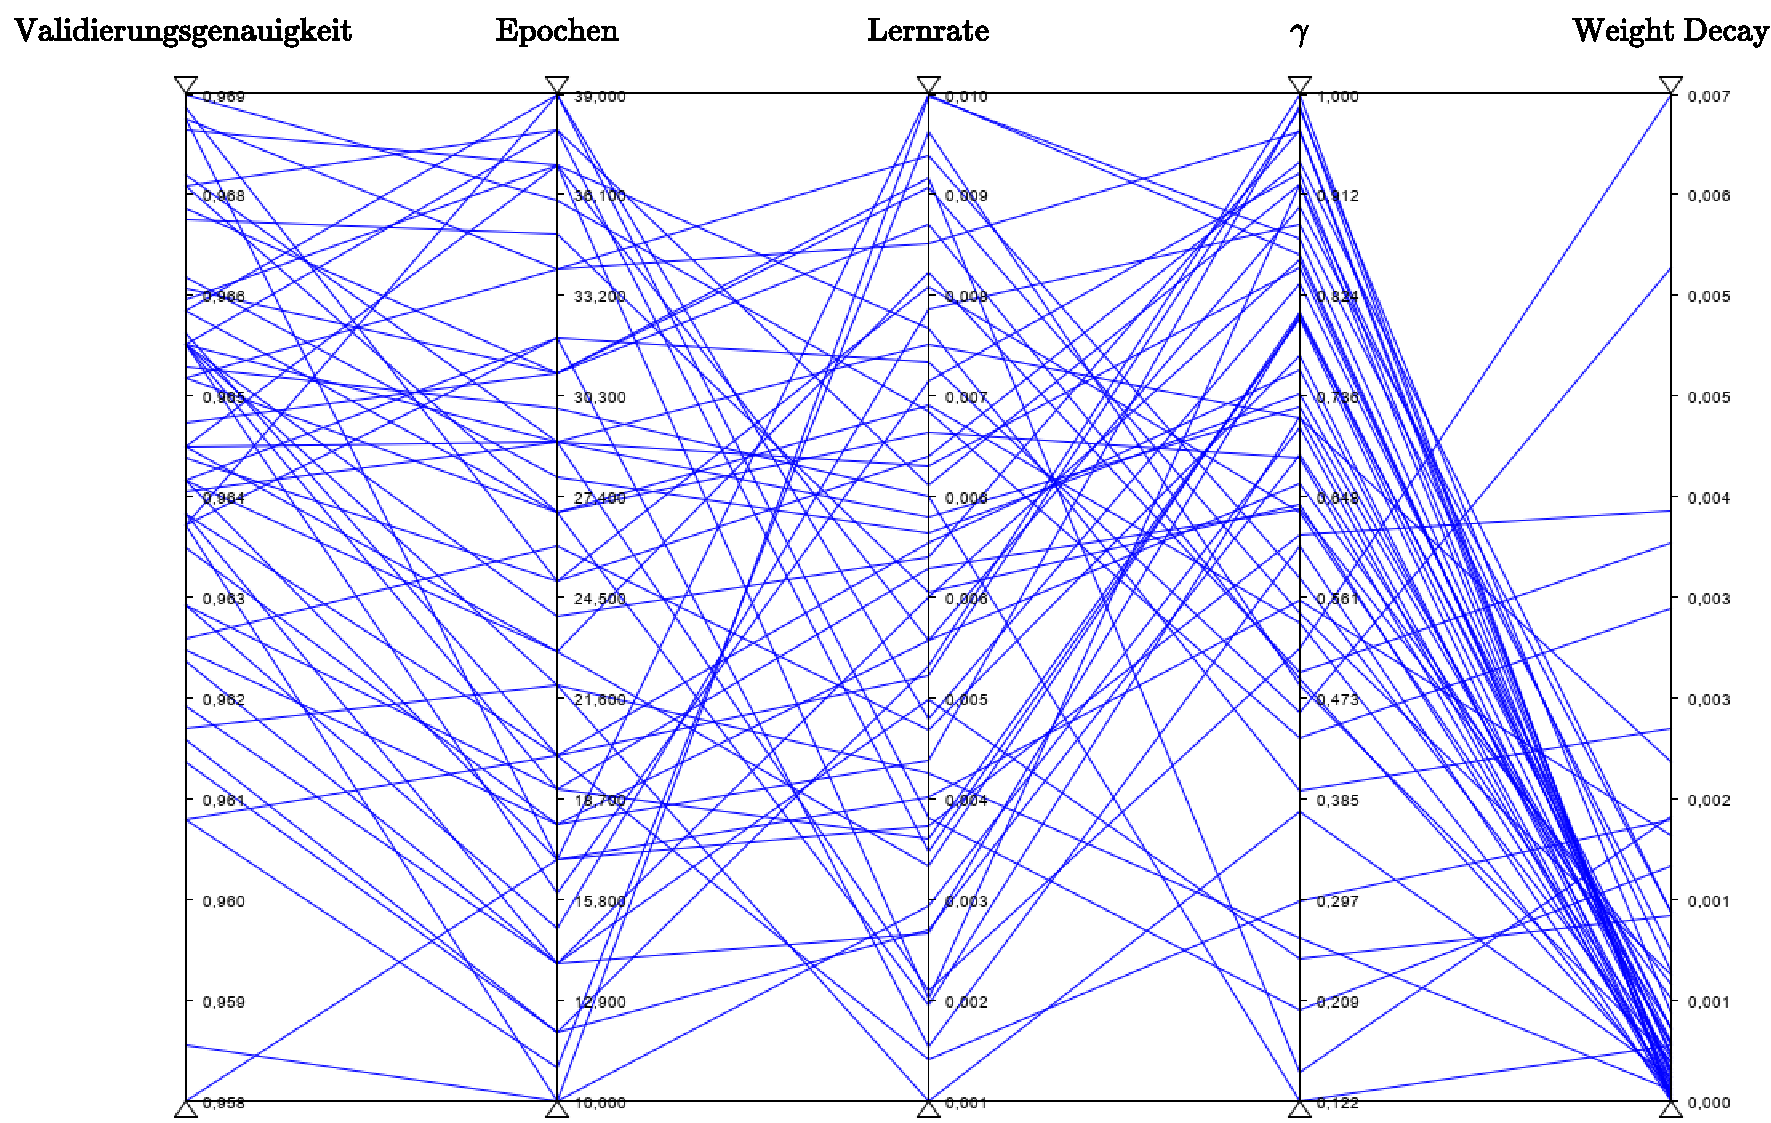
\includegraphics[scale=0.52]{NNOPT/Anhang/layer4_attention.pdf}
\caption{Parallele Darstellung der getesteten Konfigurationen des Attention-Trainings, bei Verwendung von Deskriptoren aus \mbox{Block-4}. Jede Linie repräsentiert einen Konfiguration und die von ihr erzielte Validierungsgenauigkeit.}
\label{hyperopt_layer4_2}
\end{figure}
\newpage
\begin{figure}[h]
\begin{center}


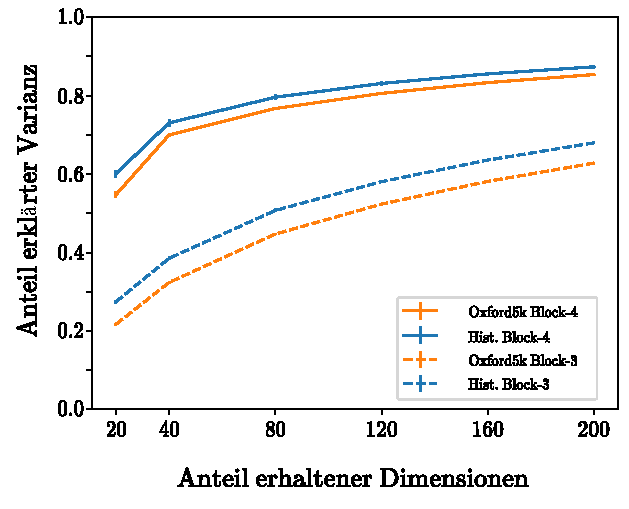
\includegraphics[scale=1.3]{NNOPT/Anhang/explained_variance_layer4}
\caption{Erklärter Anteil der Varianz nach Deskriptortransformtion durch Hauptkomponentenanalyse auf unterschiedlichen Retrievaldatensätzen, bei Verwendung von unterschiedlichen Extraktionspunkten je nach Anzahl erhaltener Dimensionen. }
\label{hyperopt_layer4_3}
\end{center}

Bei Verwendung von Deskriptoren aus Block-4 kann ein deutlich größerer Anteil der Varianz in wenigen Dimensionen abgebildet werden, als mit Deskriptoren aus Block-3. Dabei sind die größten Eigenwerte, die bei der Hauptkomponentenanalyse auf den Deskriptoren aus Block-4 berechnet wurden deutlich größer, als bei Verwendung von Deskriptoren aus Block-3. Das heißt, die ersten Hauptkomponenten/Dimensionen bilden mehr Varianz ab. Zusätzlich ist die Summe der Eigenwerte bei der Analyse der Deskriptoren aus Block-4 geringer als bei Block-3. Folglich ist die Varianz zwischen den Deskriptoren aus Block-4 geringer als zwischen den Deskriptoren aus Block-3.
\end{figure}

\begin{figure}[h]
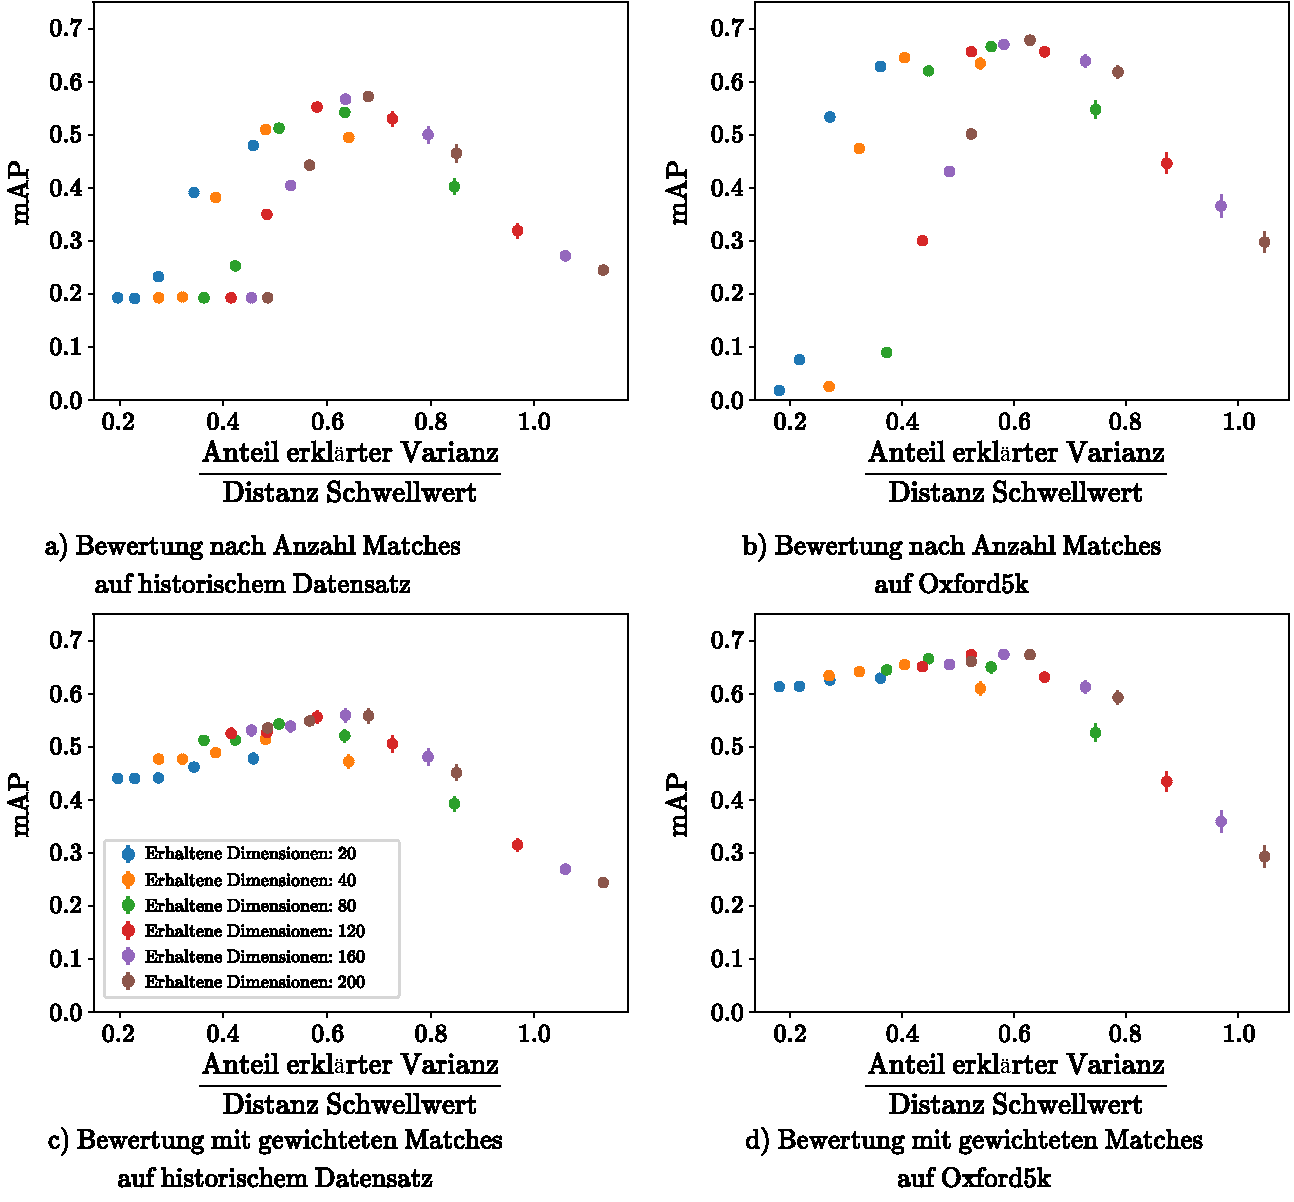
\includegraphics[scale=0.73]{mAP_var_dist_ratio_scoring_methods}
\caption{Erreichte mAP bei unterschiedlichen Verhältnissen zwischen erklärtem Varianzanteil und gewähltem Distanzschwellwert unter Verwendung alternativer Bewertungsmethoden.}
\label{mAP_var_dist_ratio_alternative_scoring}
\end{figure}
\end{document}